\documentclass[11pt]{article}
\usepackage[noindent]{settings}

\renewcommand{\Name}     {Dennis Yatunin}
\renewcommand{\Date}     {\today}
\renewcommand{\Prefix}   {Ph 20}
\renewcommand{\Title}    {Assignment 3}
\renewcommand{\Subtitle} {}

\begin{document}

For this assignment, I wrote the program \verb|diffeq.py|. This program has a function called \verb|euler()|, which uses the explicit, implicit, or symplectic Euler method to find the positions and velocities of the mass on a spring. It also has functions called \verb|x_exact()| and \verb|v_exact()|, which return values for the position and velocity that are found analytically.

\section*{Part 1}
I chose to set the initial position of the mass to 1, and I chose to set its initial velocity to 2. I then plotted the positions and velocities obtained with the explicit and implicit Euler methods over the time interval $[0, 15)$, using a step size of 0.05 (see Figure \ref{fig:positionsAndVelocities1}).

I then worked out the analytical solutions for the position and velocity as a function of time. Both $x = \cos(t)$ and $x = \sin(t)$ have the property that $\frac{d^2x}{dt^2} = -x$. Since $\cos(t)$ and $\sin(t)$ are linearly independent, this means that the position must have the form $x = C_1\cos(t) + C_2\sin(t)$, where $C_1, C_2 \in \mathbb{R}$ are constants. Using the conditions that $x\bigr|_{t = 0} = 1$ and $\frac{dx}{dt}\bigr|_{t = 0} = 2$ tells us that $C_1 = 1$ and $C_2 = 2$. Thus, we get that $x = \cos(t) + 2\sin(t)$ and $\frac{dx}{dt} = 2\cos(t) - \sin(t)$. I used this information to plot the errors in the positions and velocities obtained using the explicit and implicit Euler methods (see Figure \ref{fig:errors}).

The correct value for the energy given the initial conditions is $x^2 + \bigl(\frac{dx}{dt}\bigr)^2 = 5\cos^2(t) + 5\sin^2(t) = 5$. However, the energy obtained with the explicit Euler method is only 5 when $t = 0$, and it increases superlinearly as $t$ increases, approaching $\infty$ in the limit of $t \to \infty$. The energy obtained with the implicit Euler method is also 5 when $t = 0$, but it decreases sublinearly as $t$ increases, approaching 0 in the limit of $t \to \infty$ (see Figure \ref{fig:energy1}). Because the energy obtained using these methods is monotonically increasing or decreasing for all values of $t$, the errors in position and velocity grow larger in magnitude as $t$ increases.

\vfill

\begin{figure}[H]
    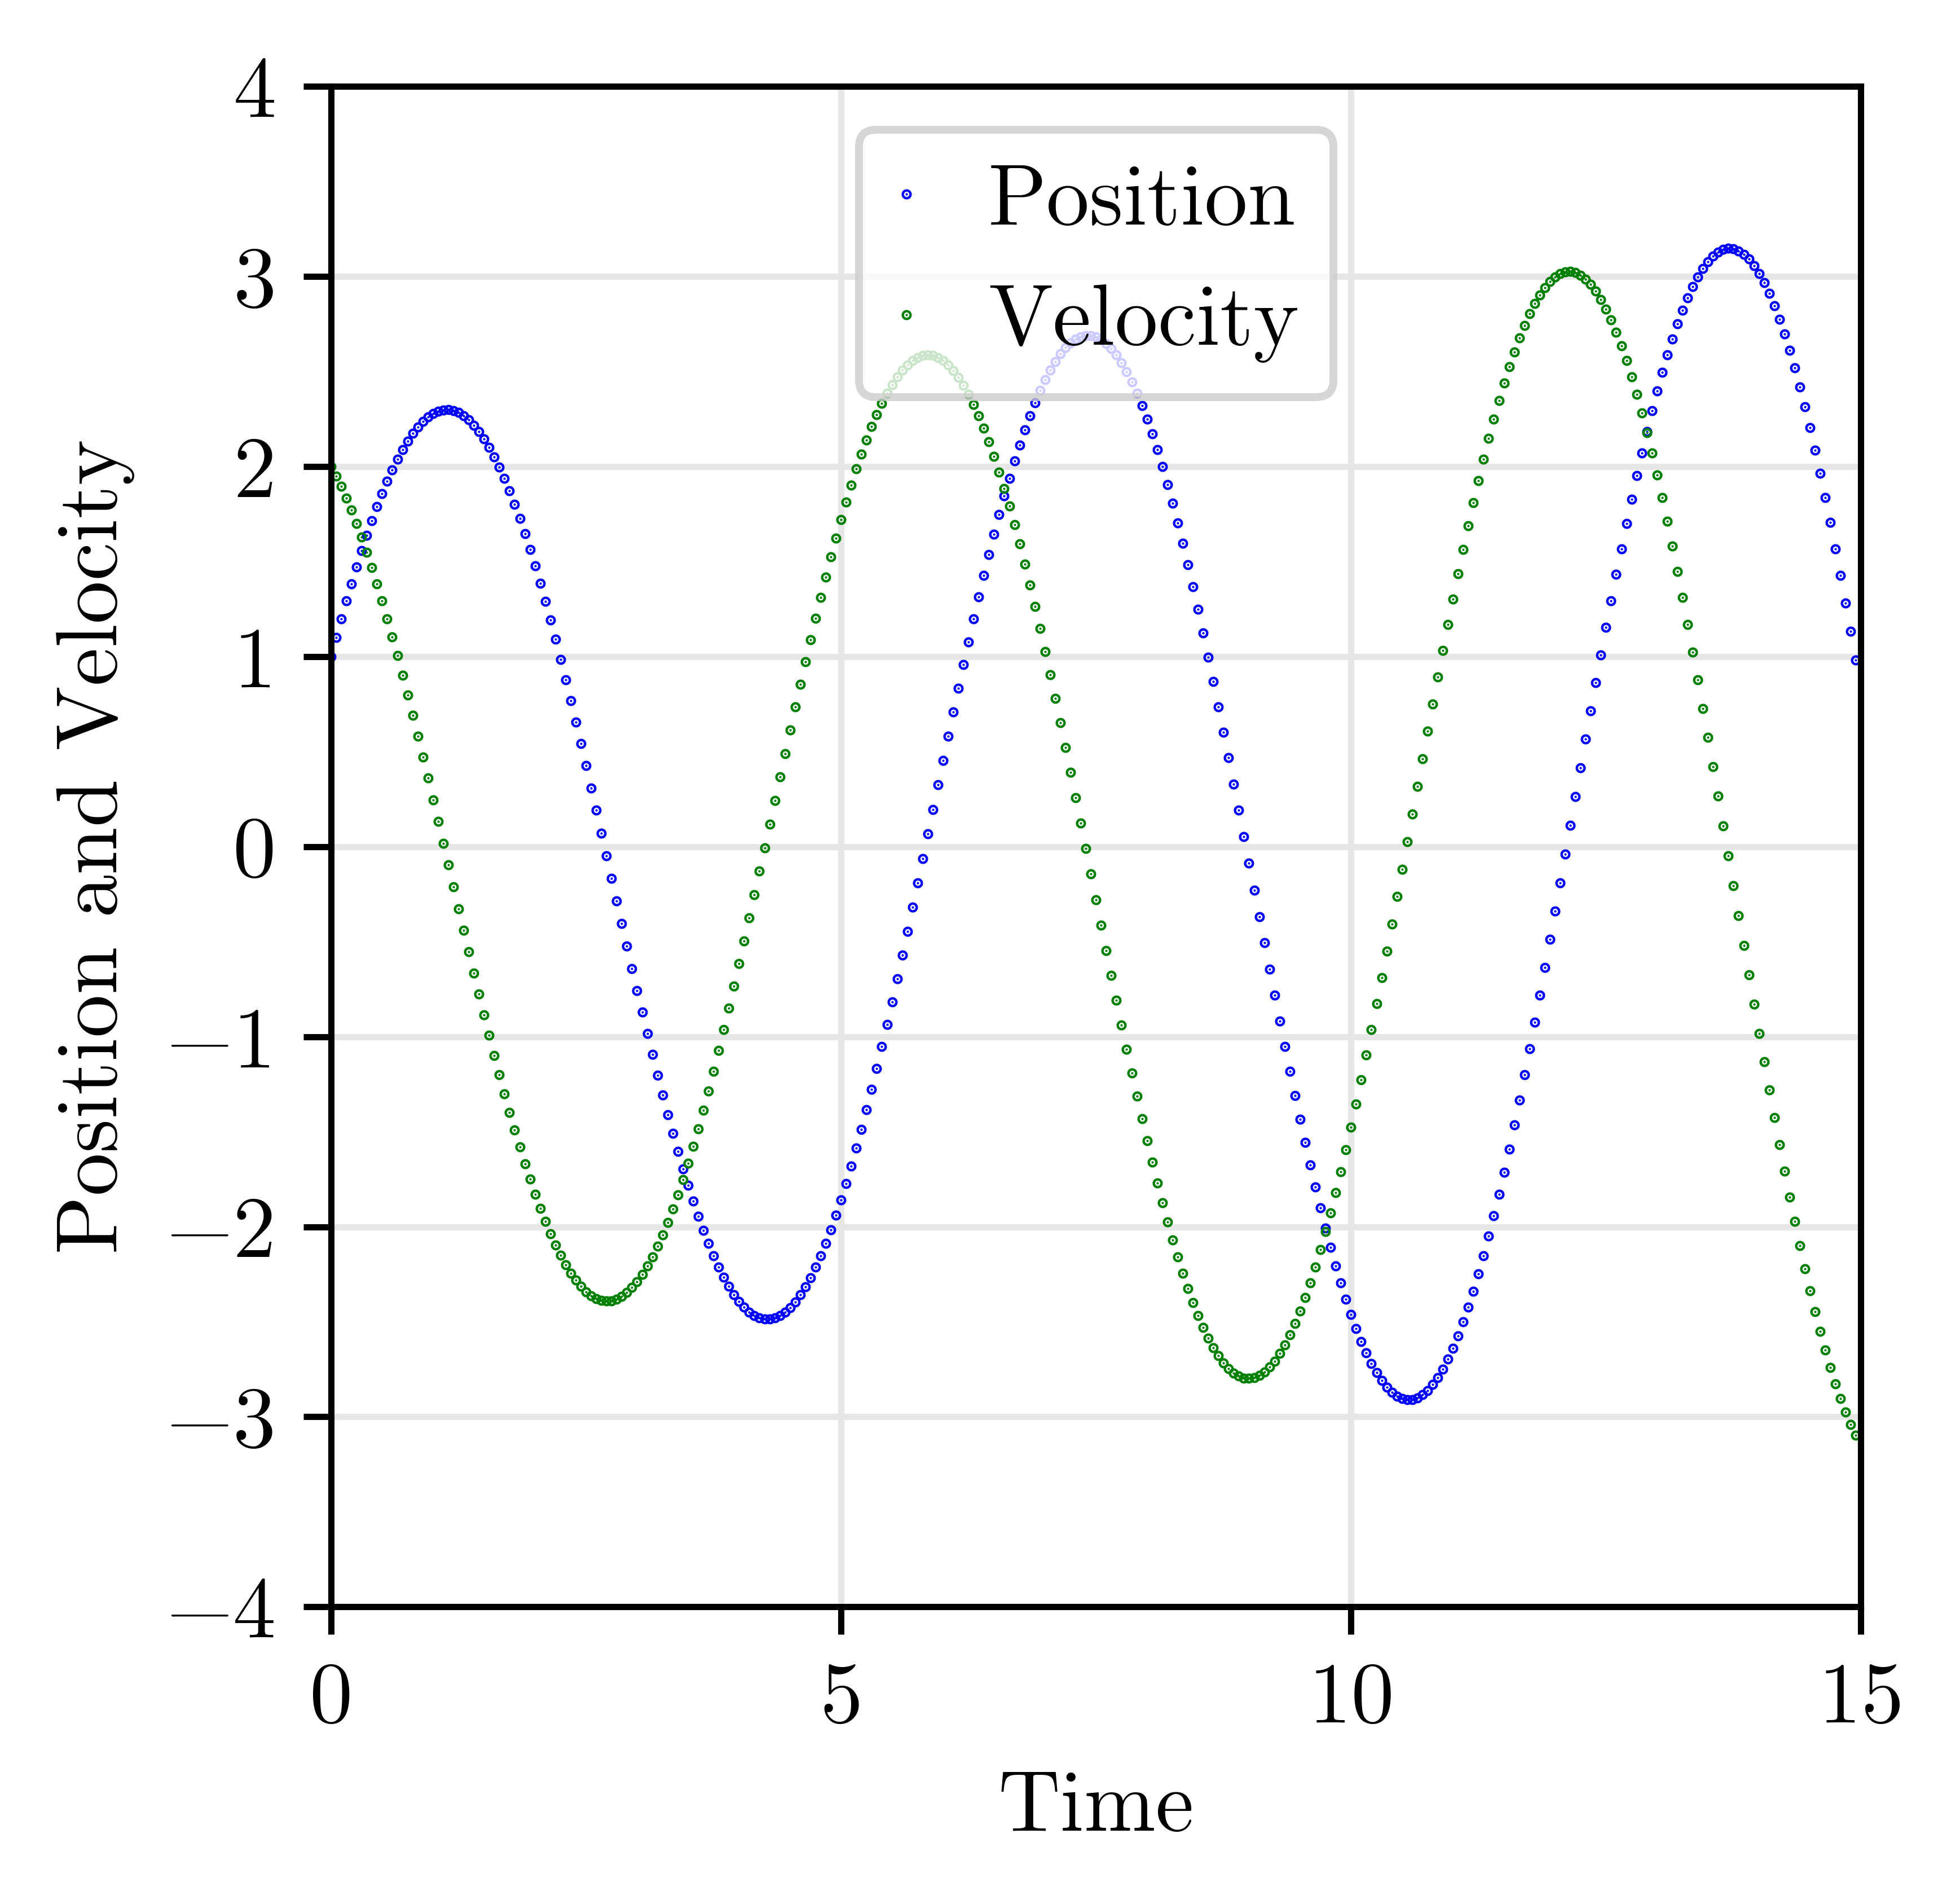
\includegraphics{explicit_euler} \hspace{0.7em} 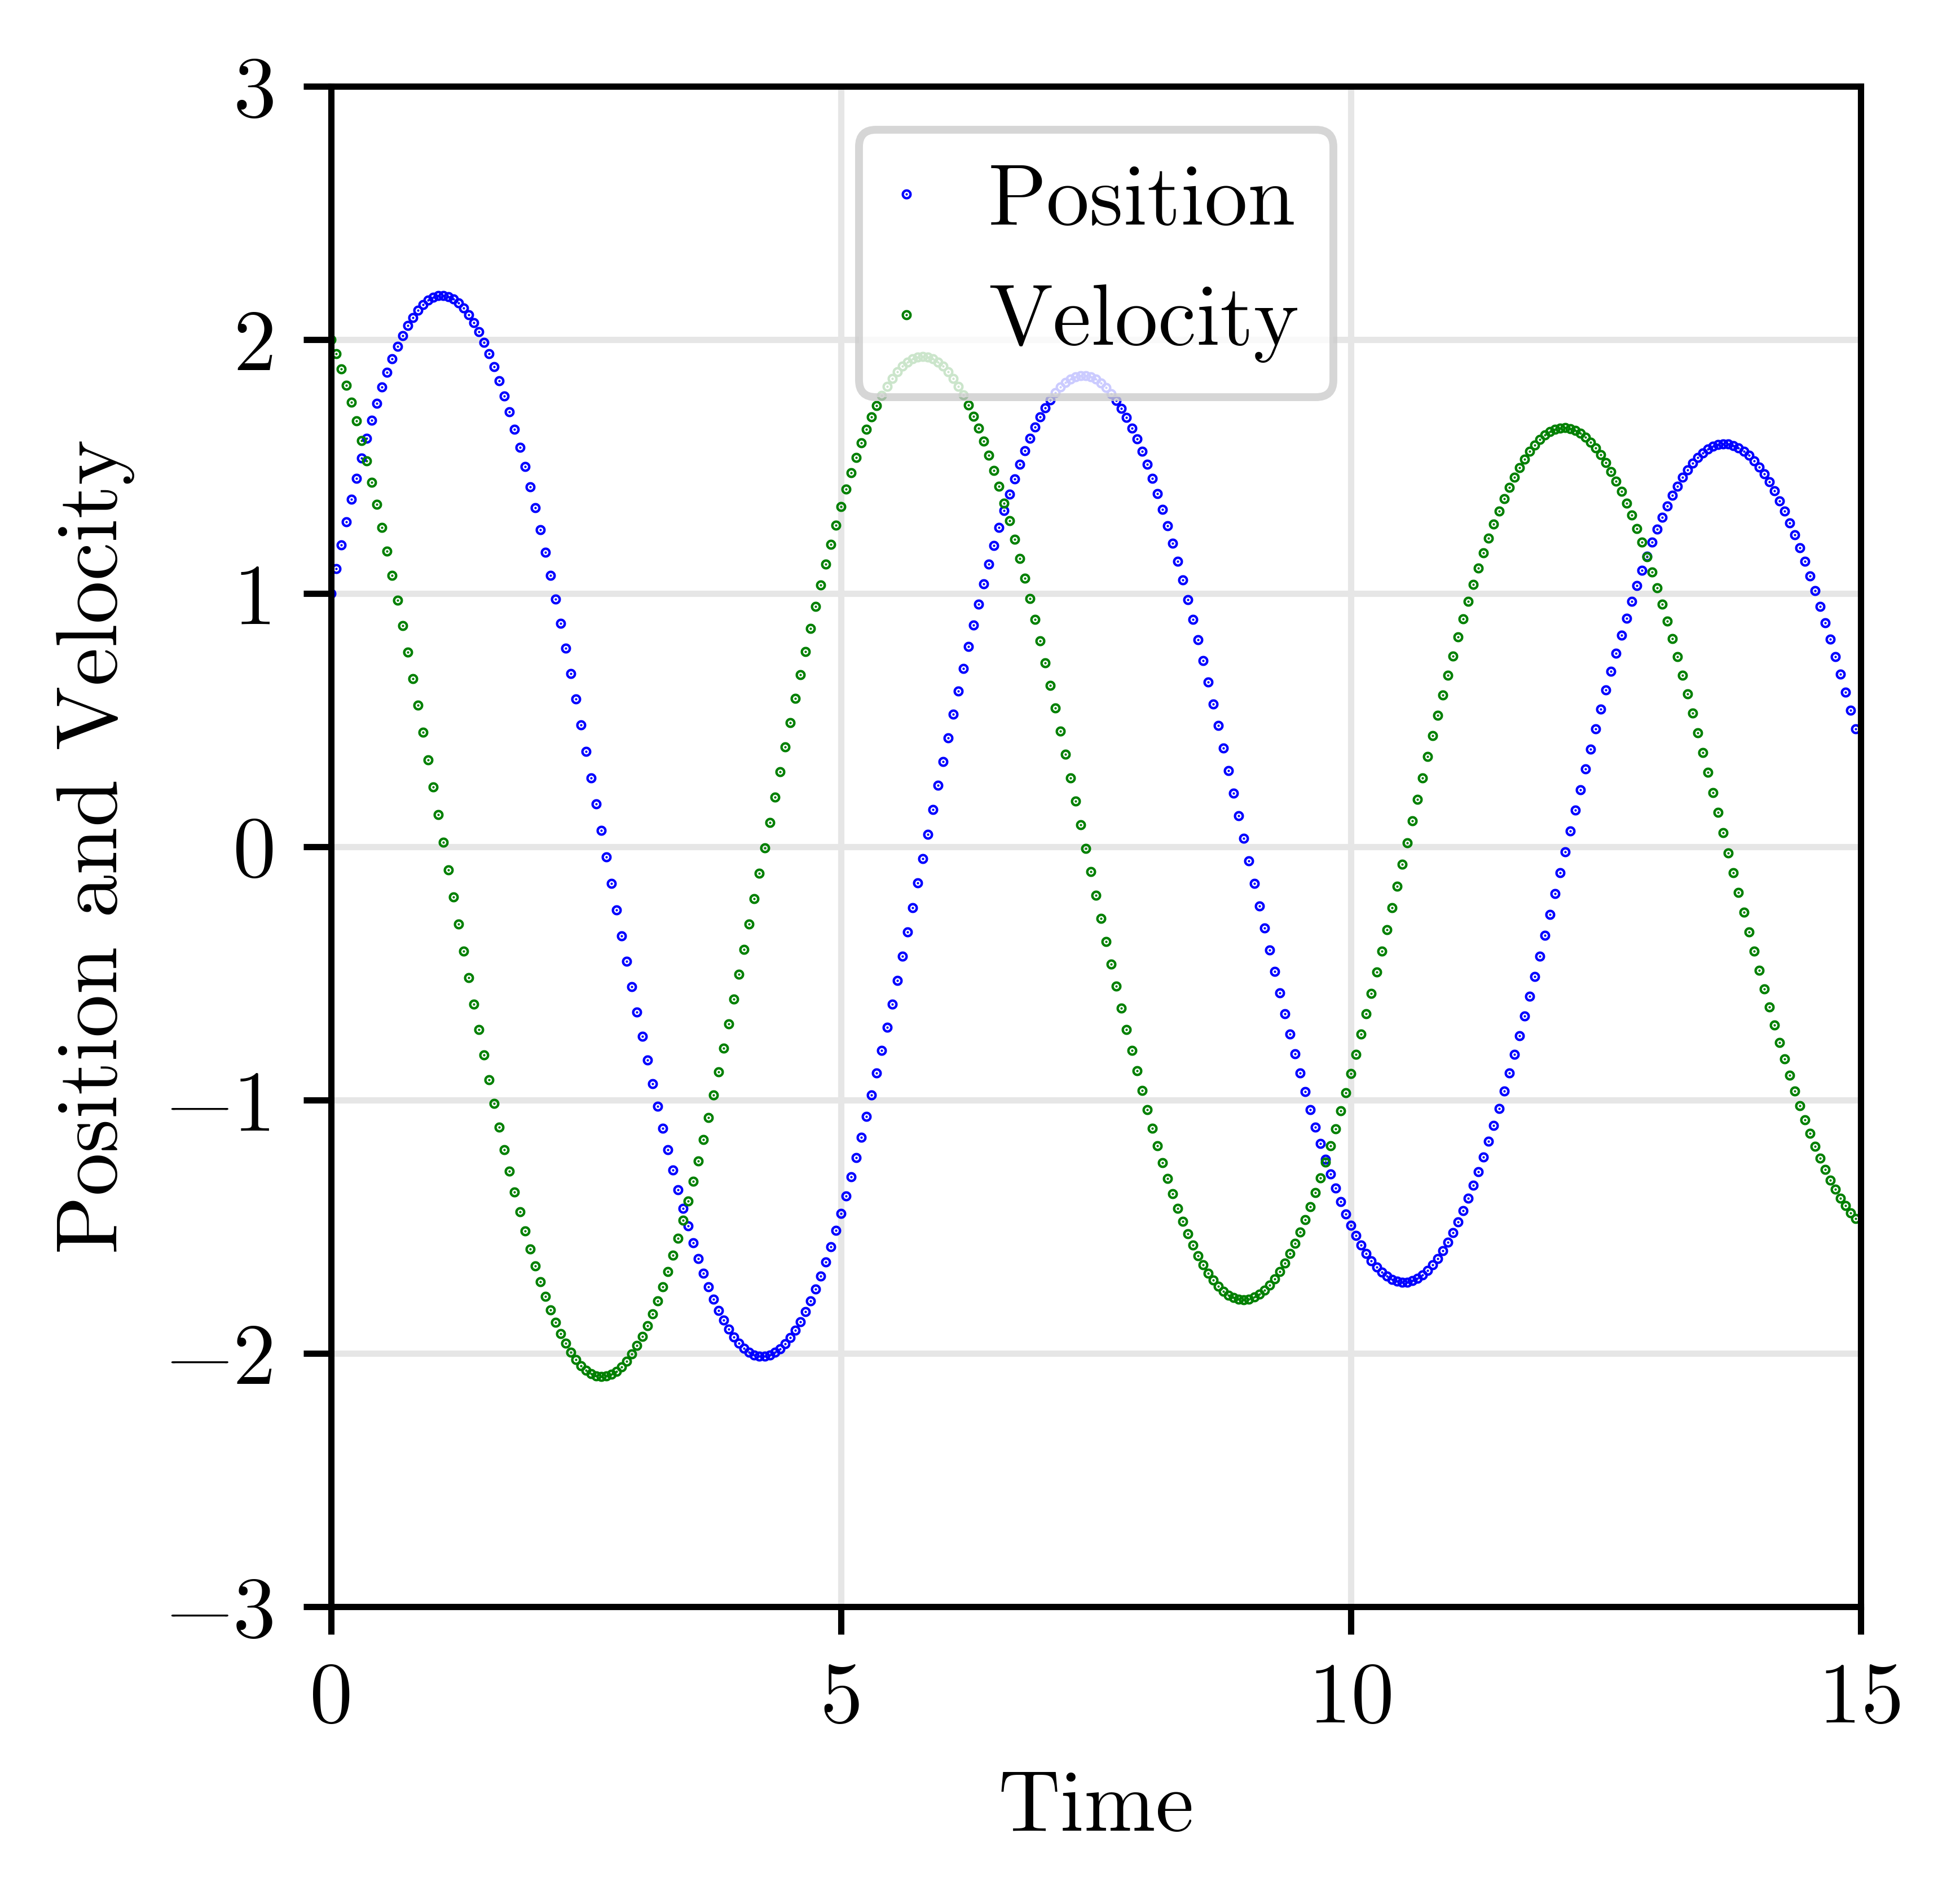
\includegraphics{implicit_euler}\\
    \caption{(Left) The positions and velocities of the mass on a spring obtained with the explicit Euler method, using a step size of 0.05. (Right) The positions and velocities obtained with the implicit Euler method, using a step size of 0.05.}
    \label{fig:positionsAndVelocities1}
\end{figure}

\begin{figure}[H]
    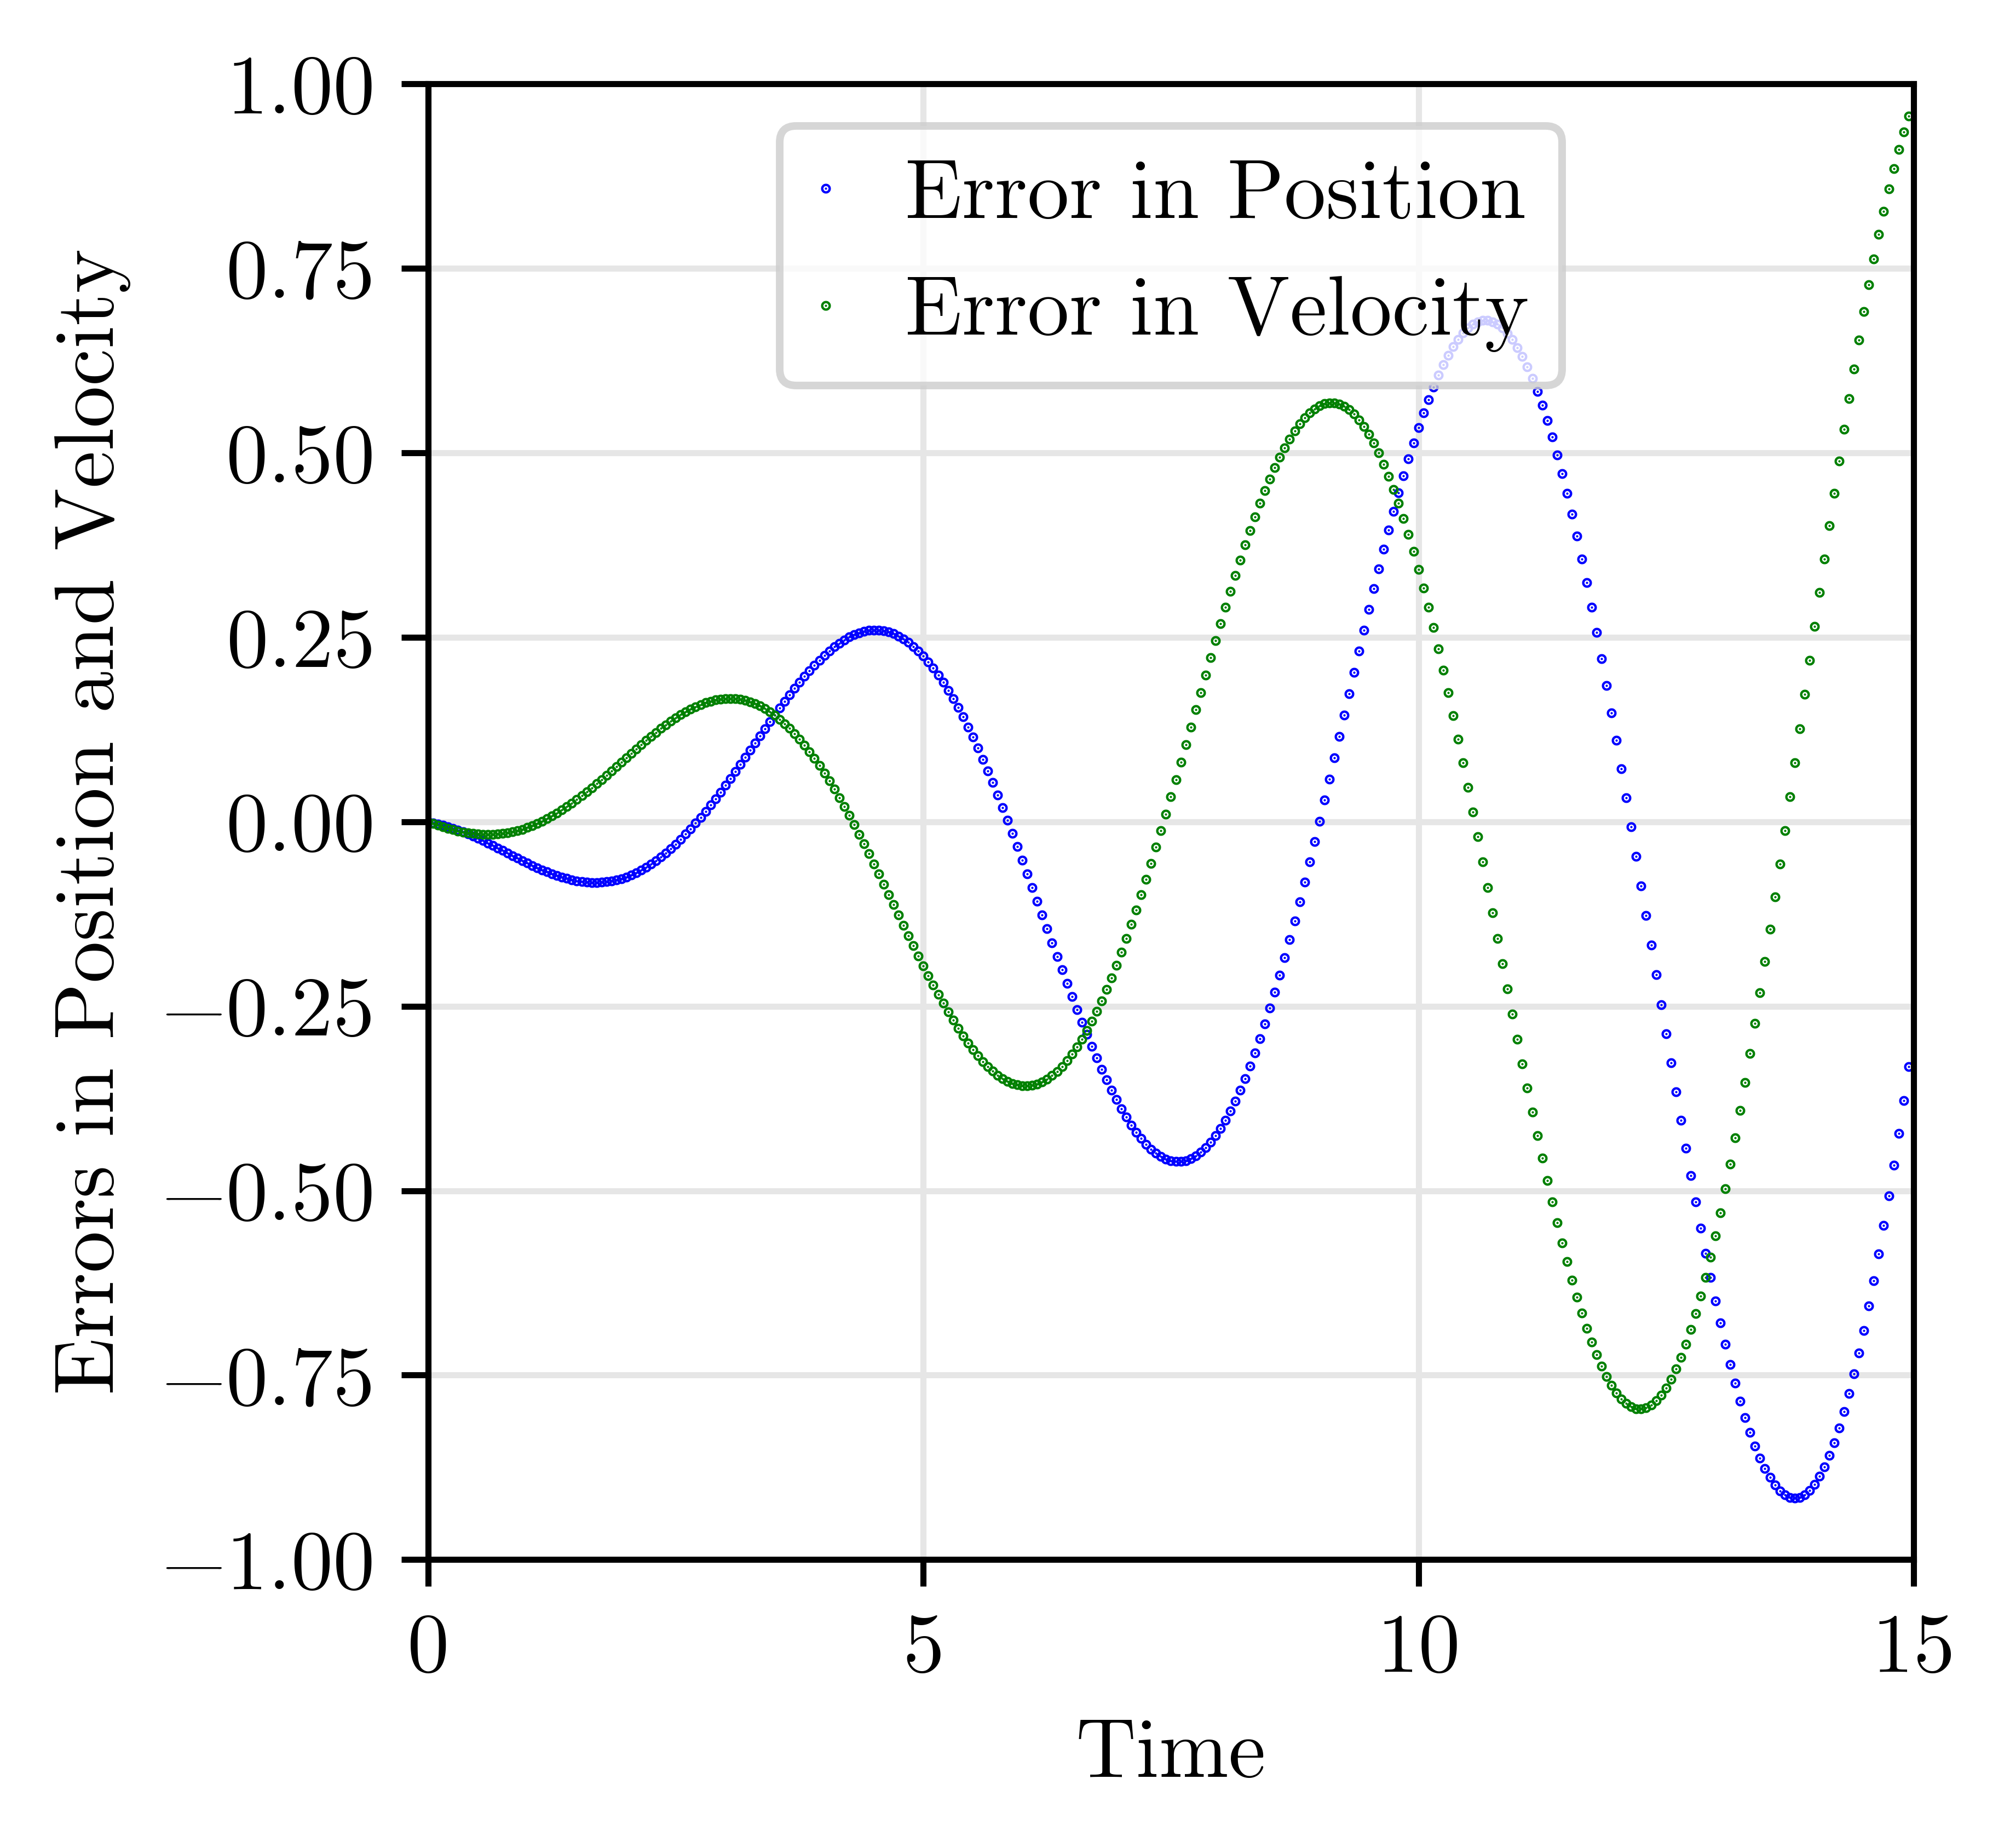
\includegraphics{explicit_euler_errors} \hspace{0.7em} 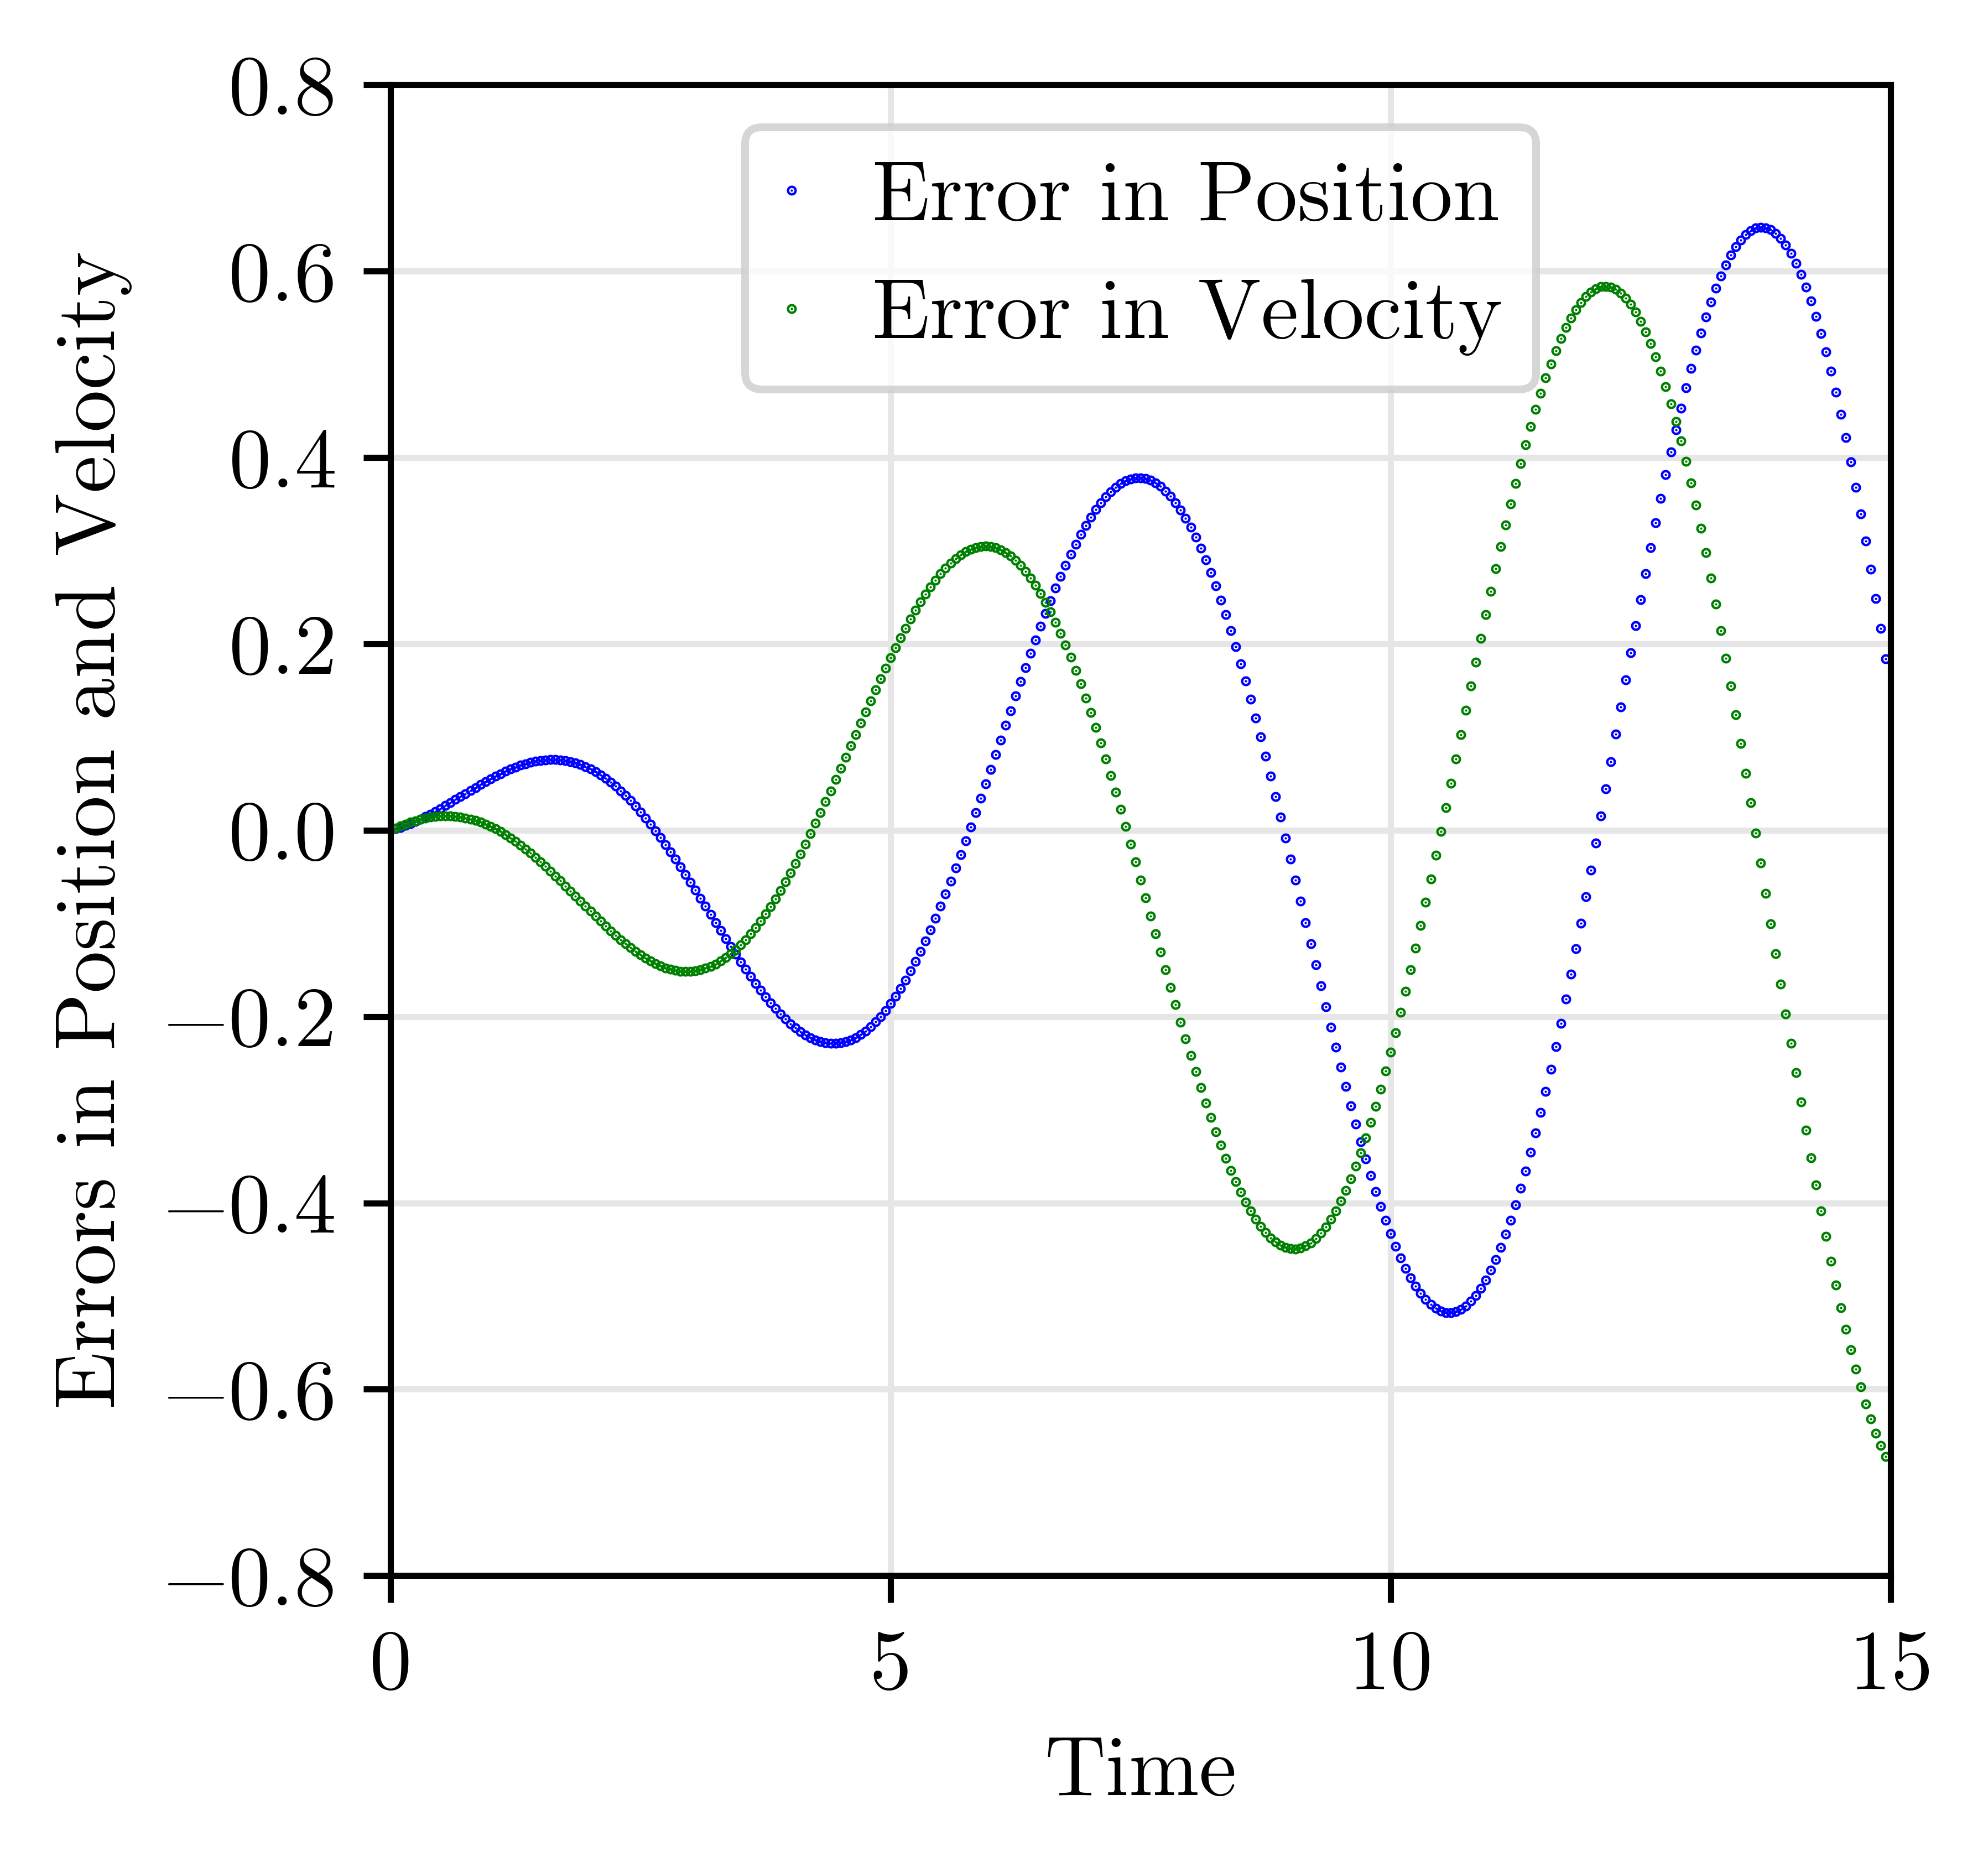
\includegraphics{implicit_euler_errors}\\
    \caption{(Left) The errors in the positions and velocities obtained with the explicit Euler method, using a step size of 0.05. (Right) The errors in the positions and velocities obtained with the implicit Euler method, using a step size of 0.05.}
    \label{fig:errors}
\end{figure}

\vfill

\begin{figure}[H]
    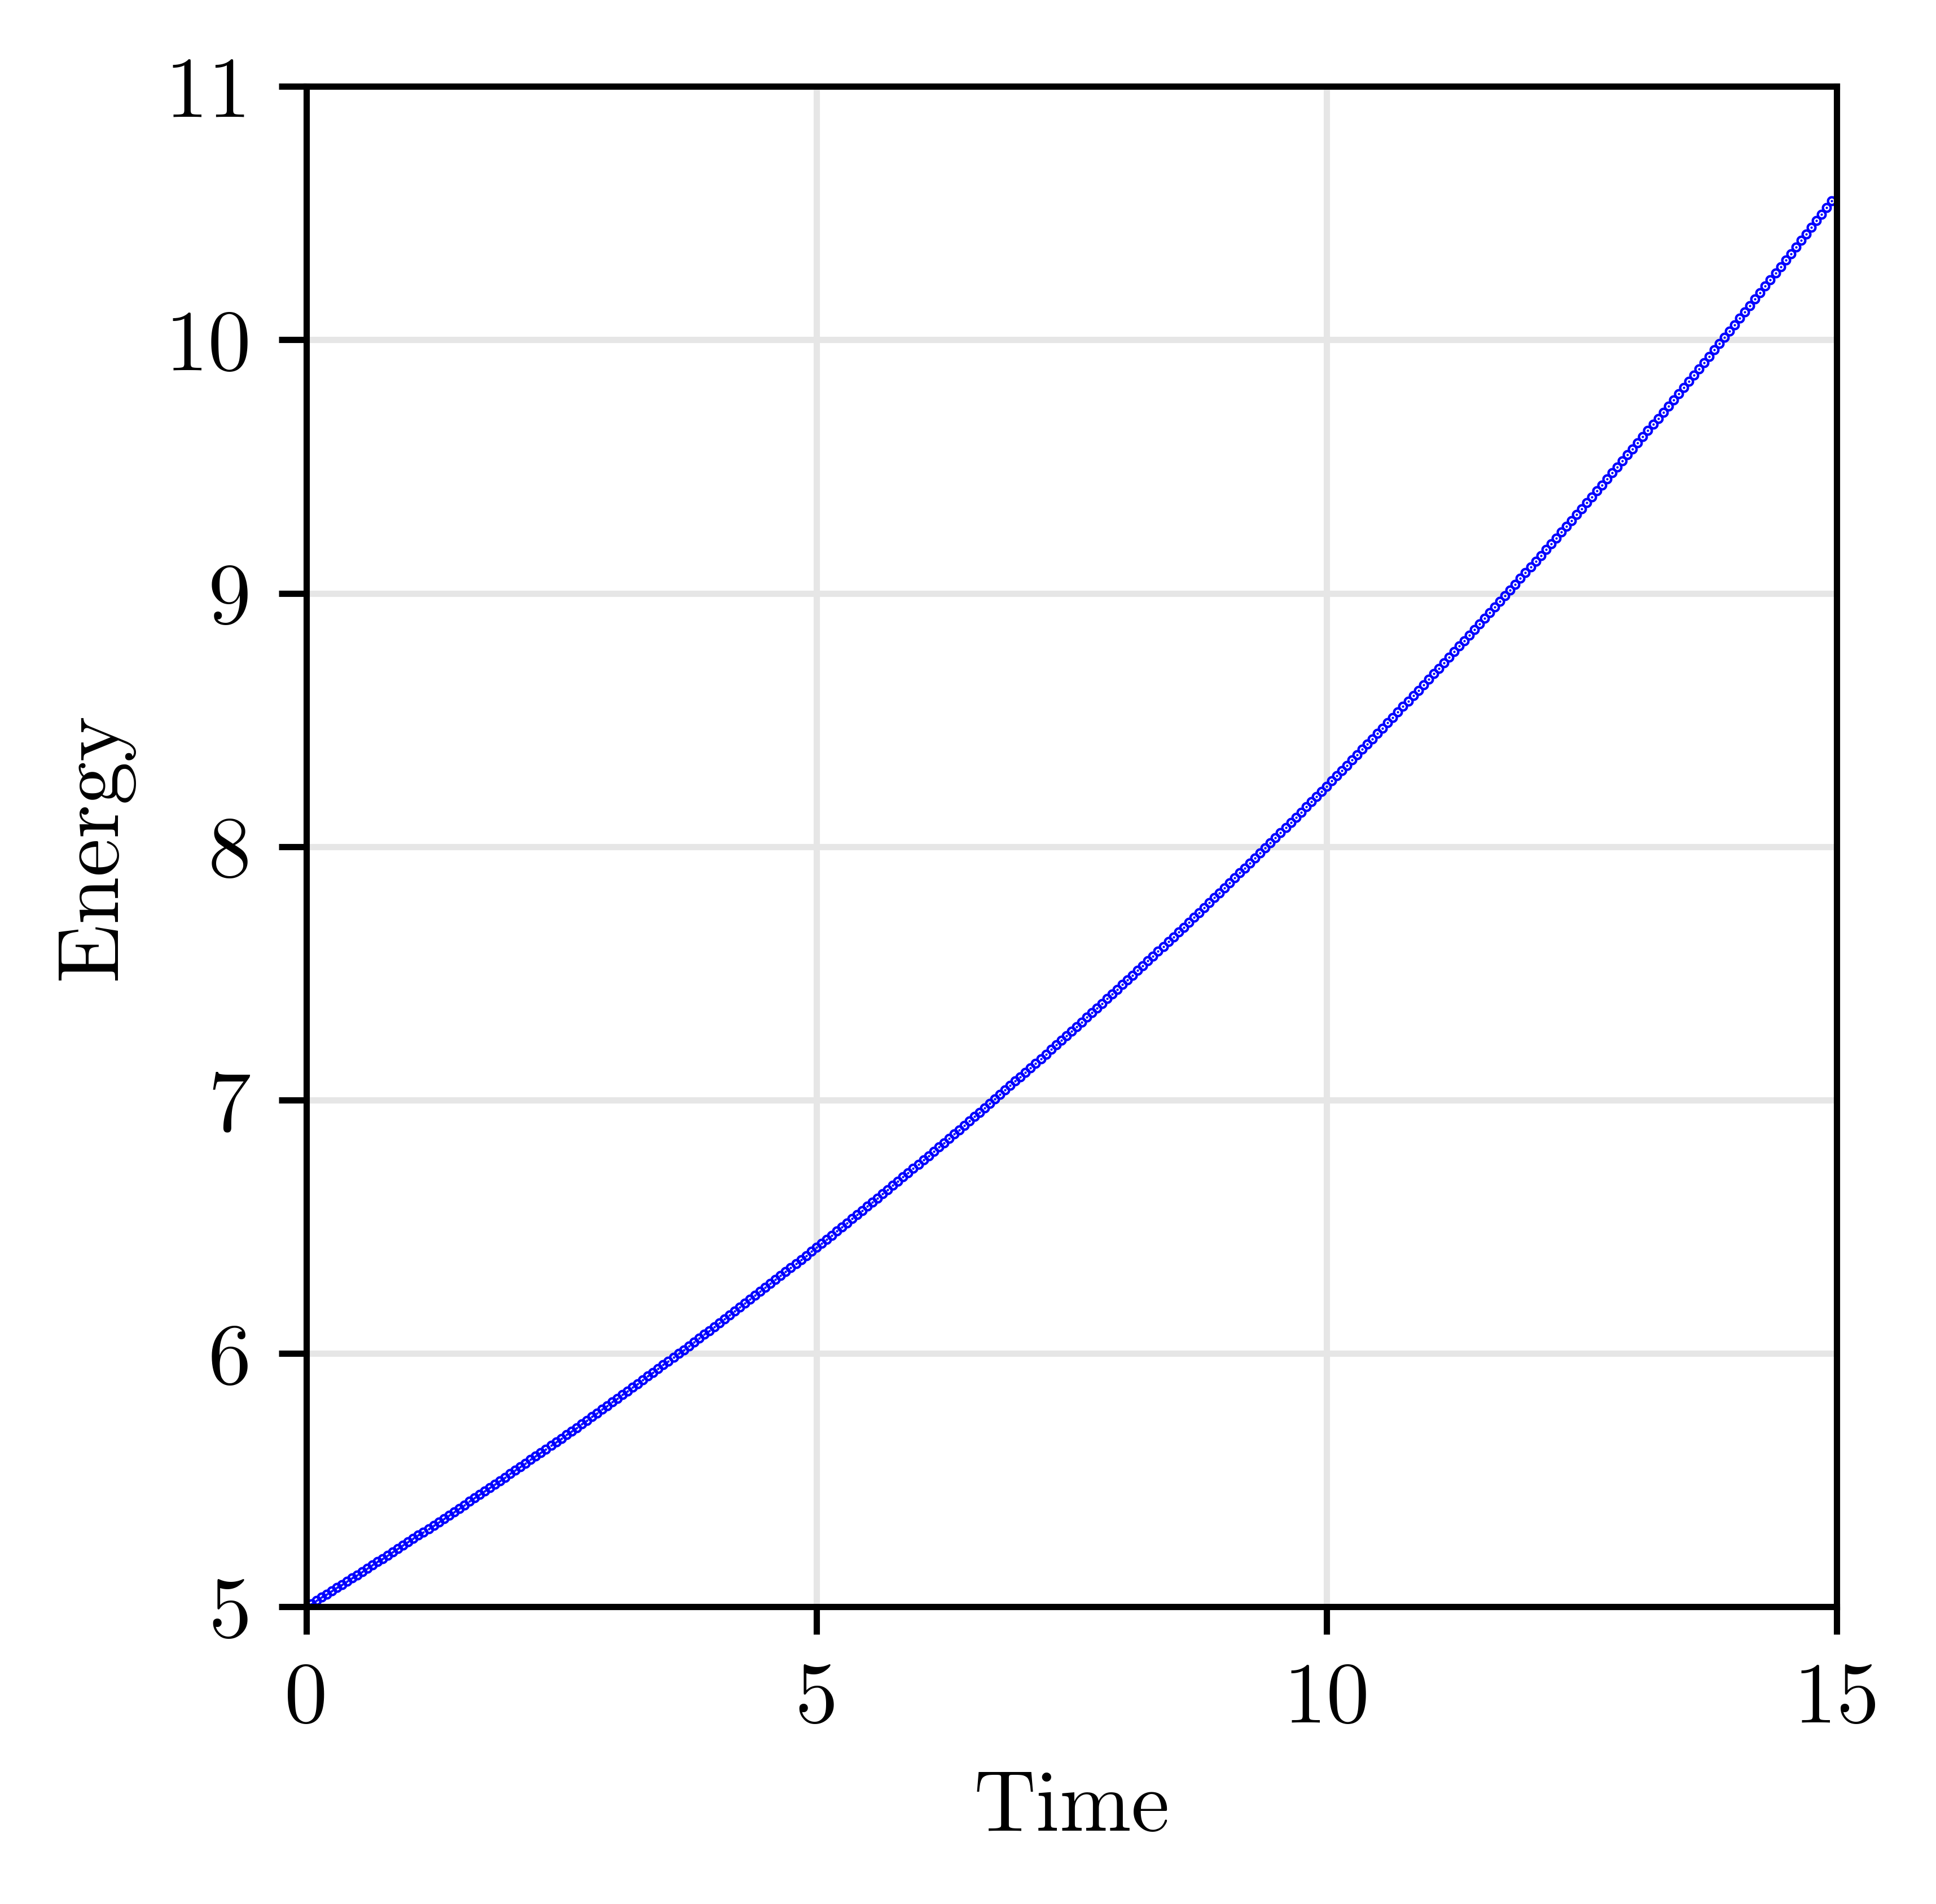
\includegraphics{explicit_euler_energy} \hspace{0.7em} 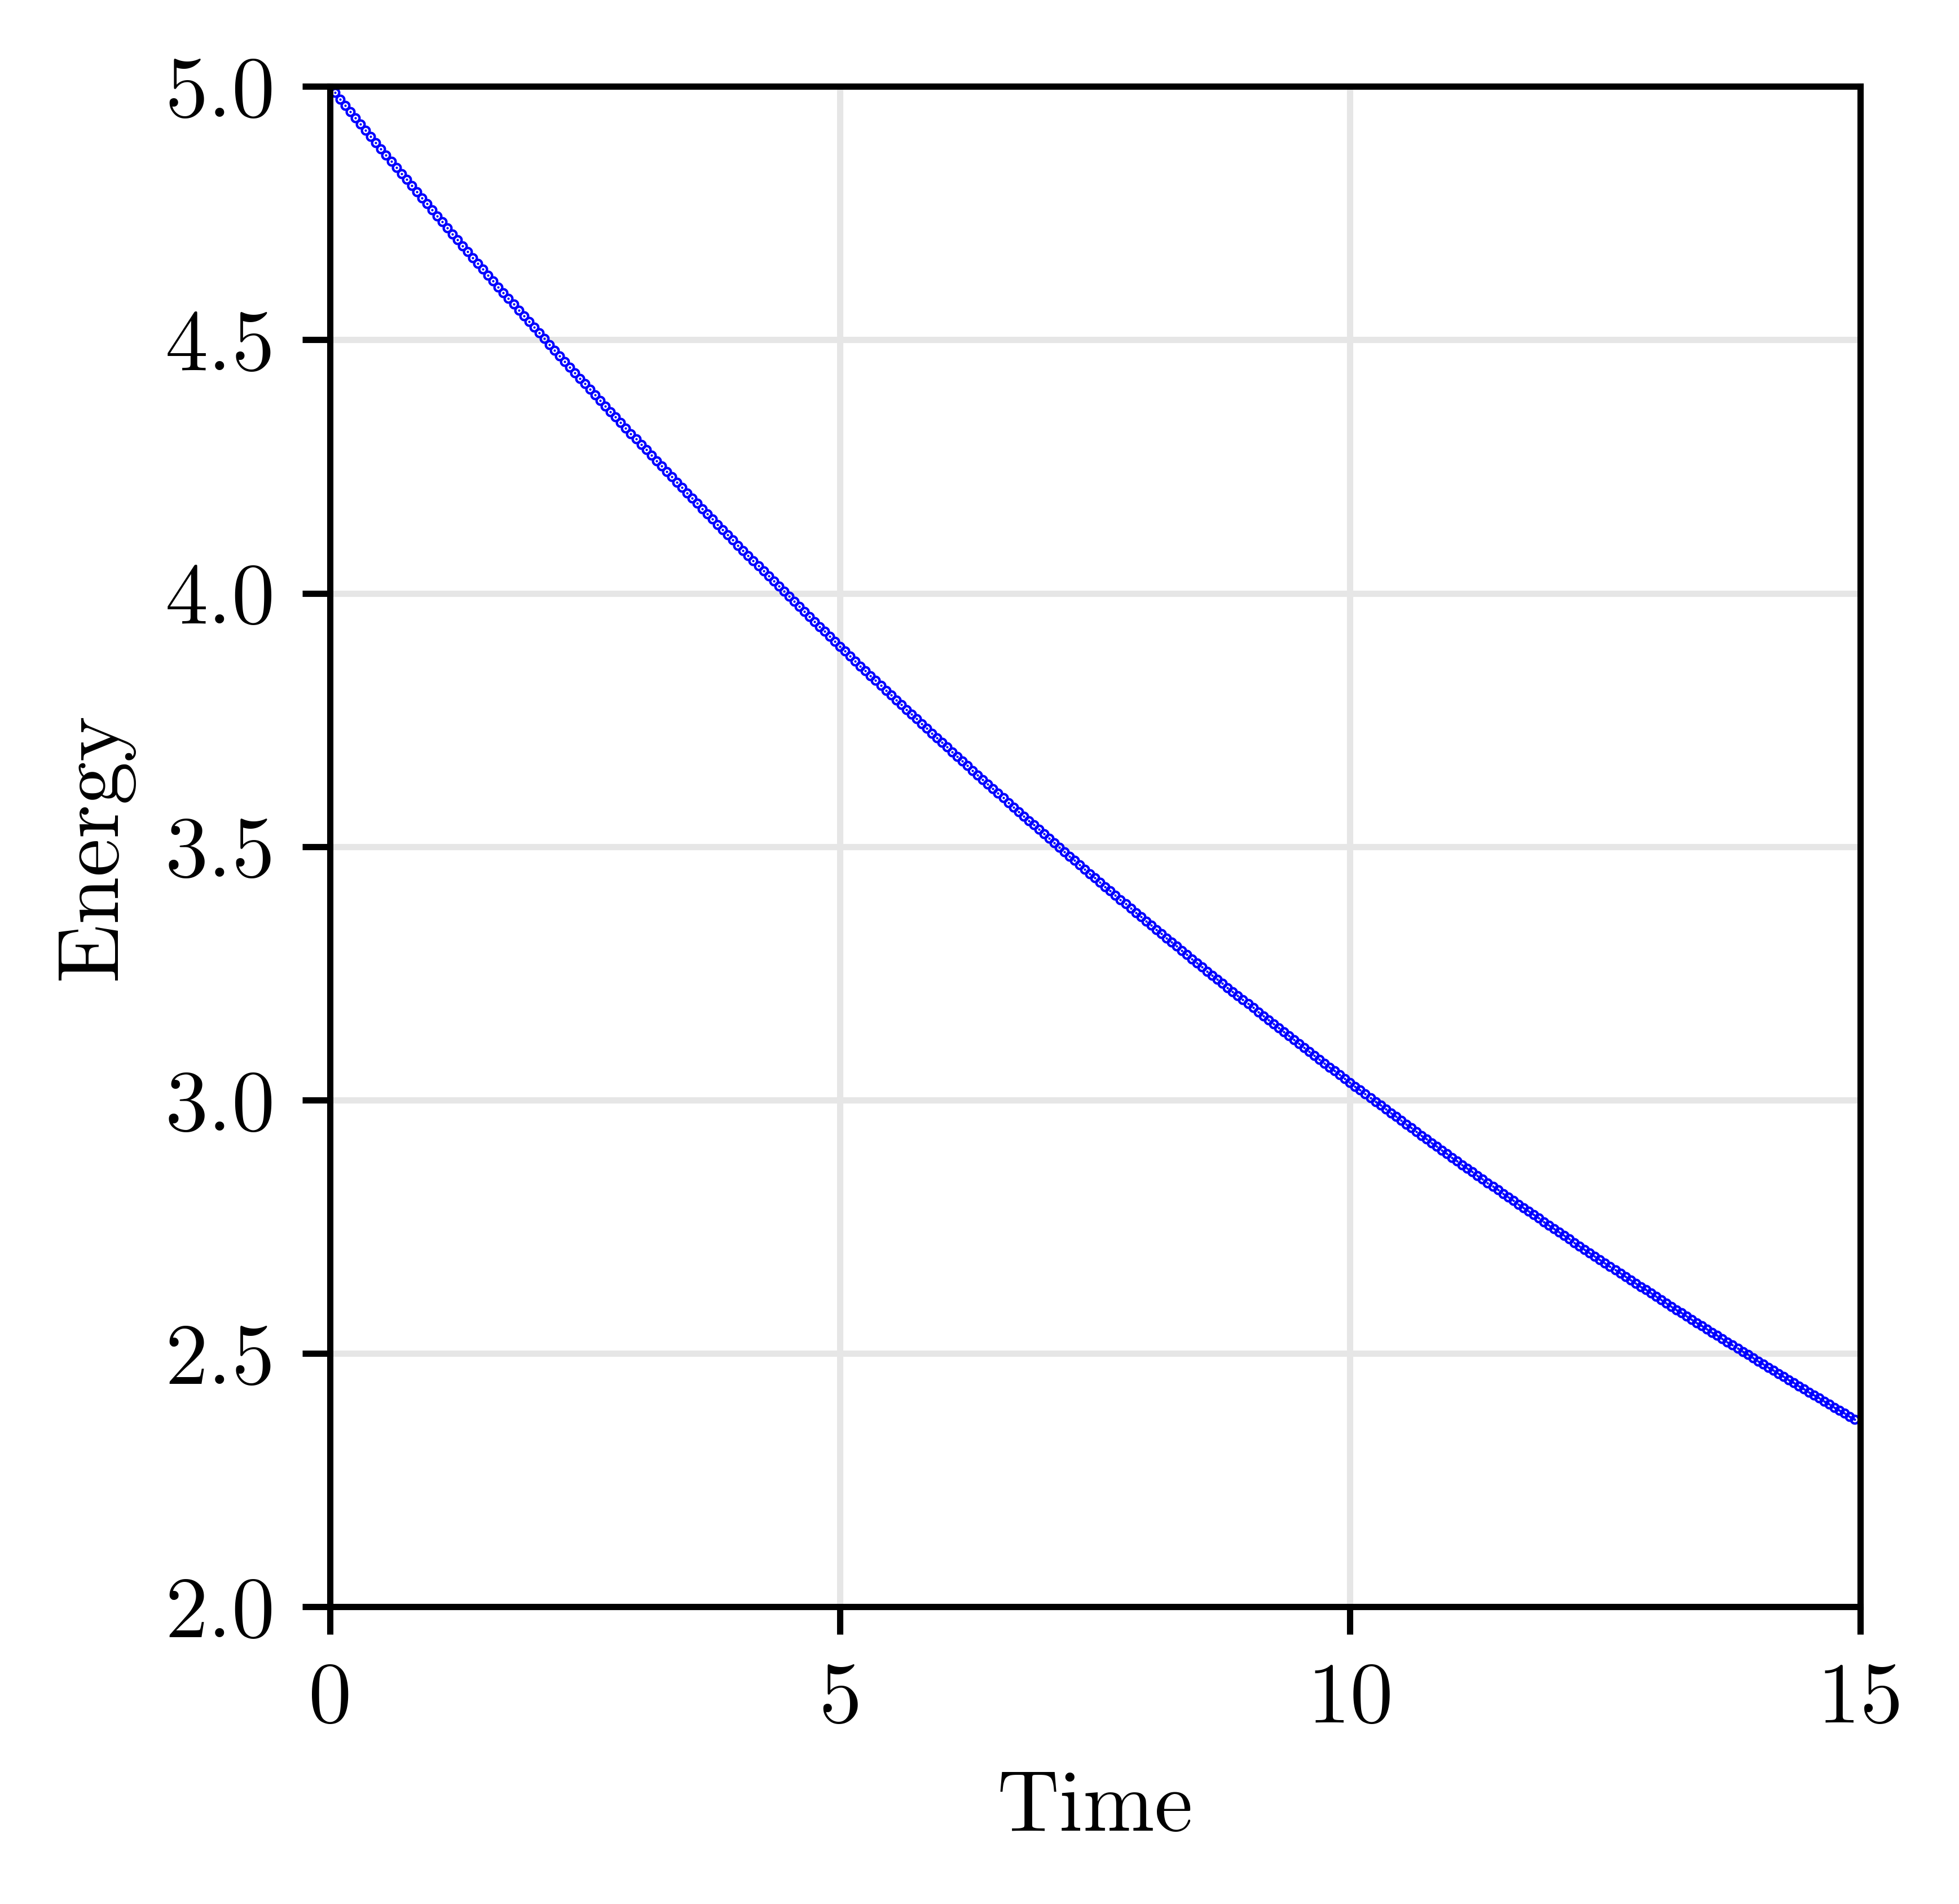
\includegraphics{implicit_euler_energy}\\
    \caption{(Left) The energy obtained with the explicit Euler method, using a step size of 0.05. (Right) The energy obtained with the implicit Euler method, using a step size of 0.05.}
    \label{fig:energy1}
\end{figure}

\begin{figure}[H]
    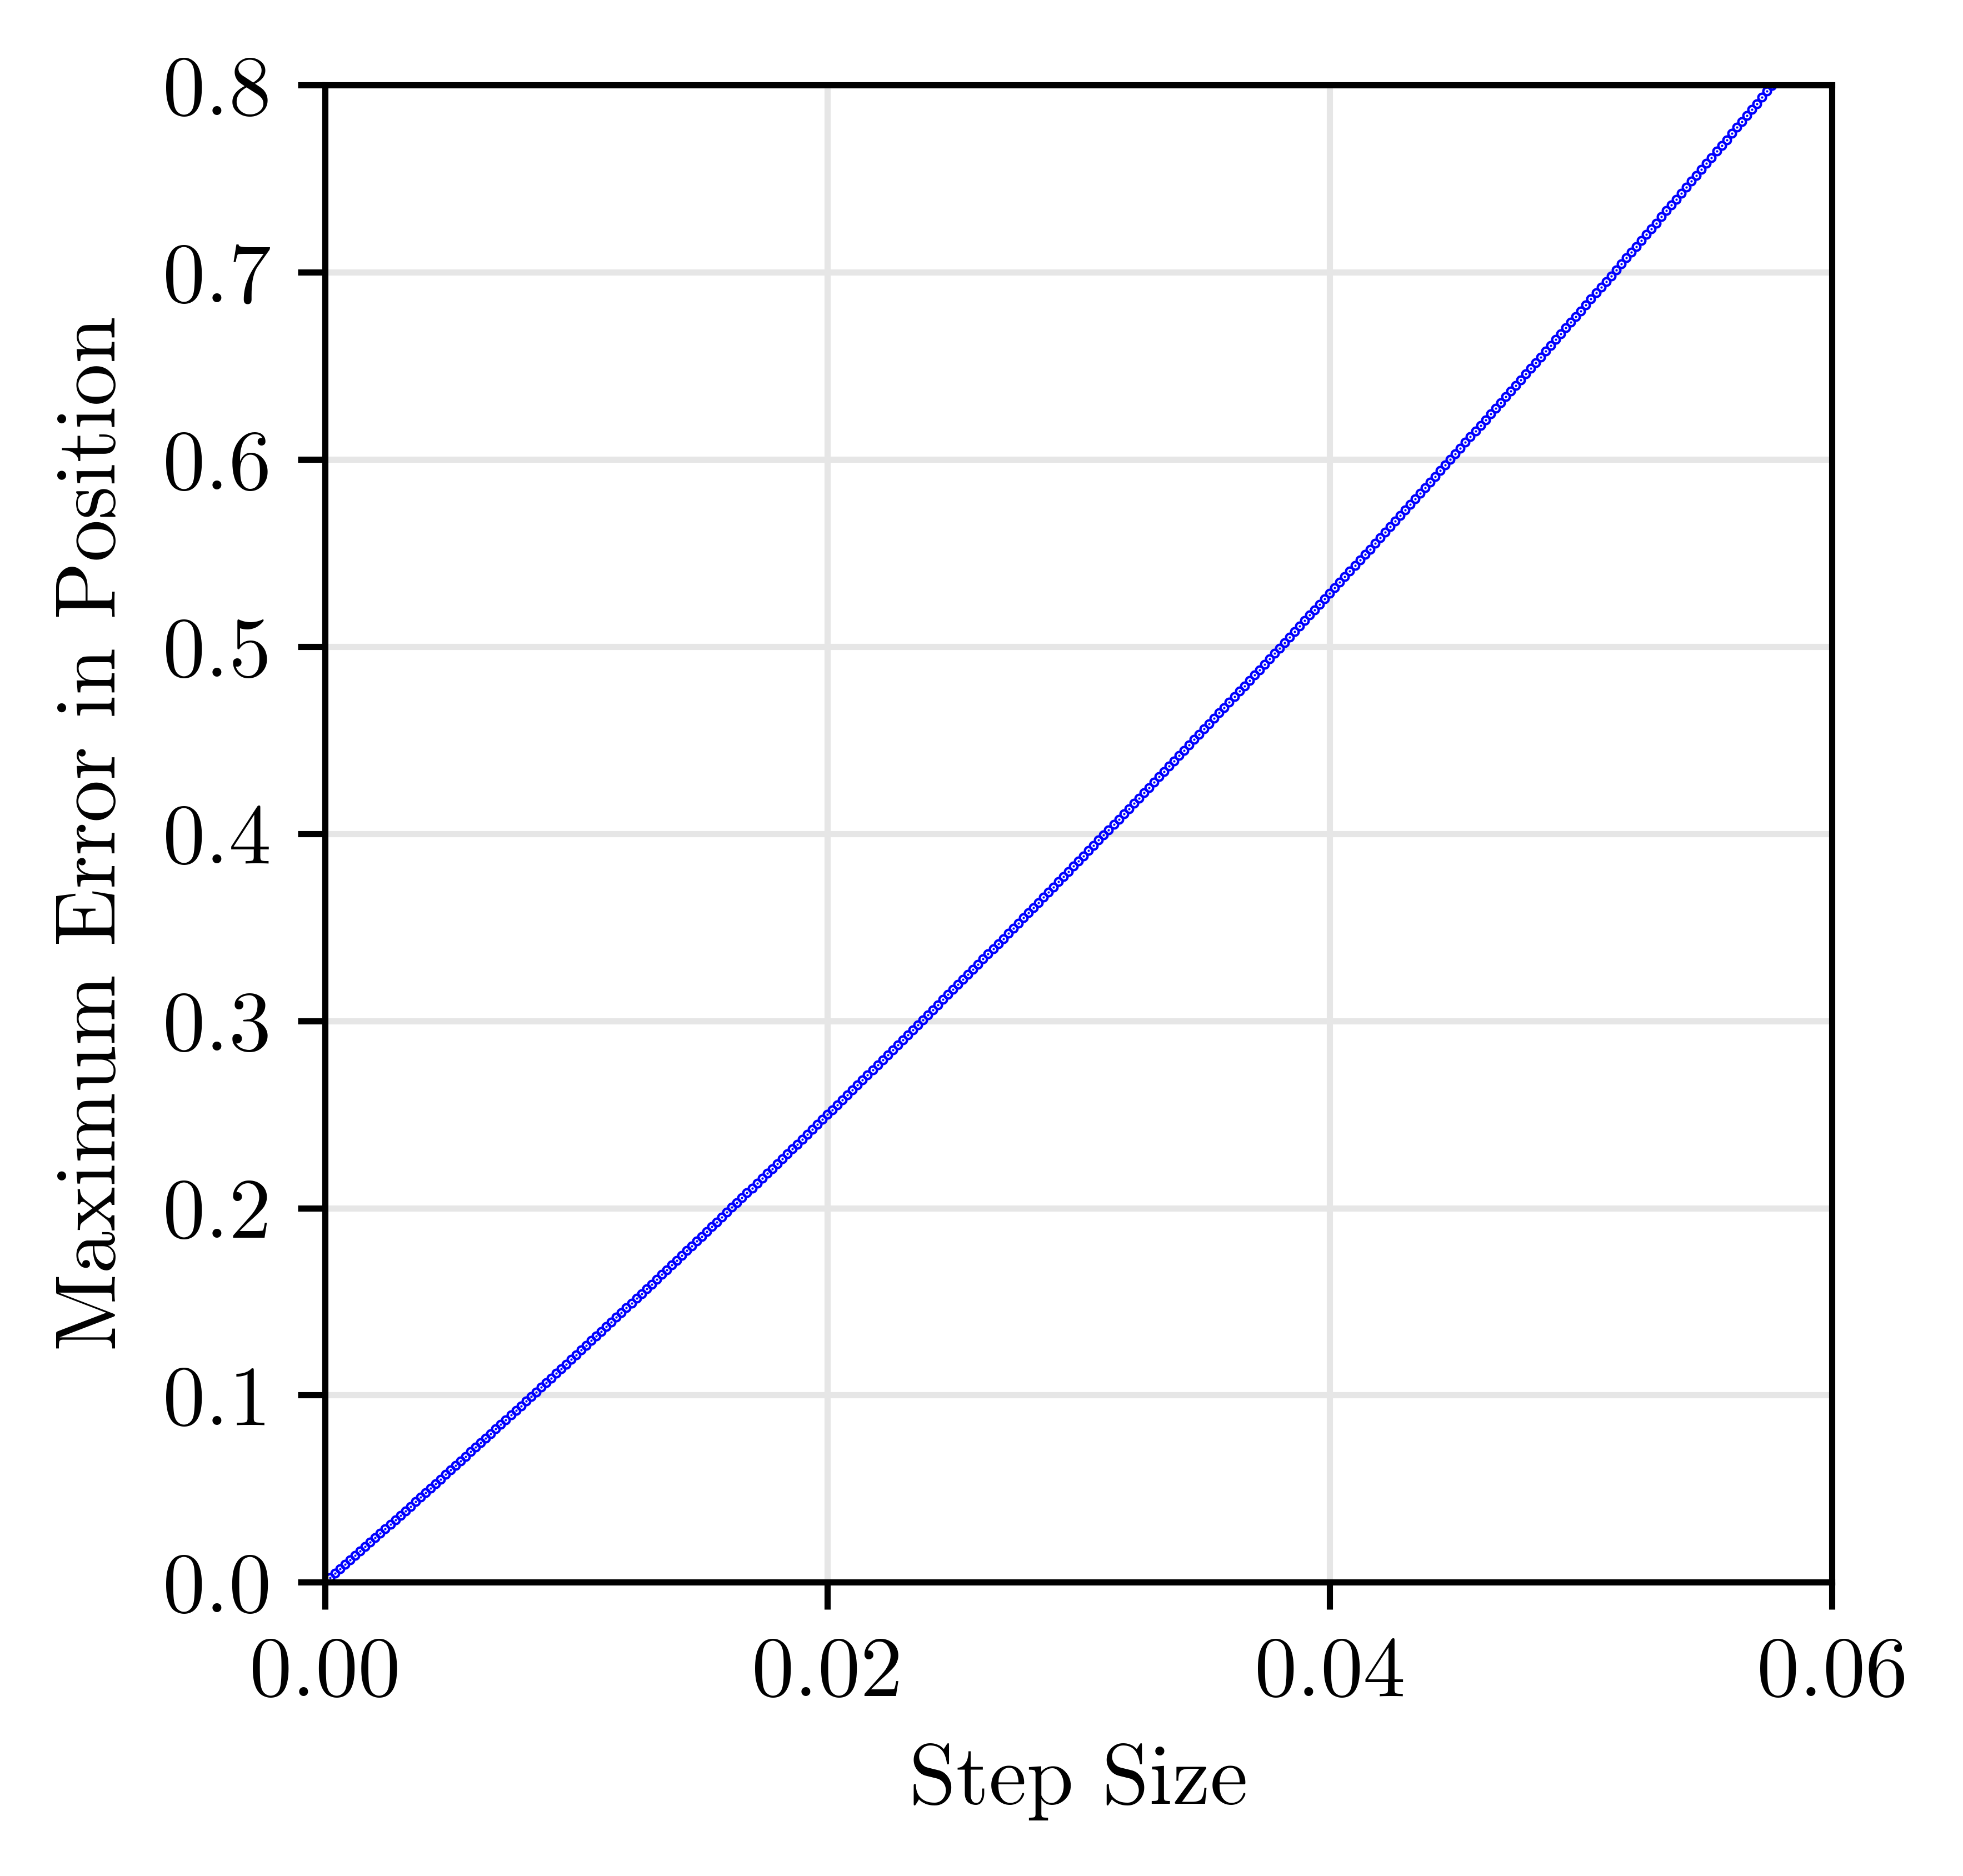
\includegraphics{explicit_euler_max_errors} \hspace{0.7em} 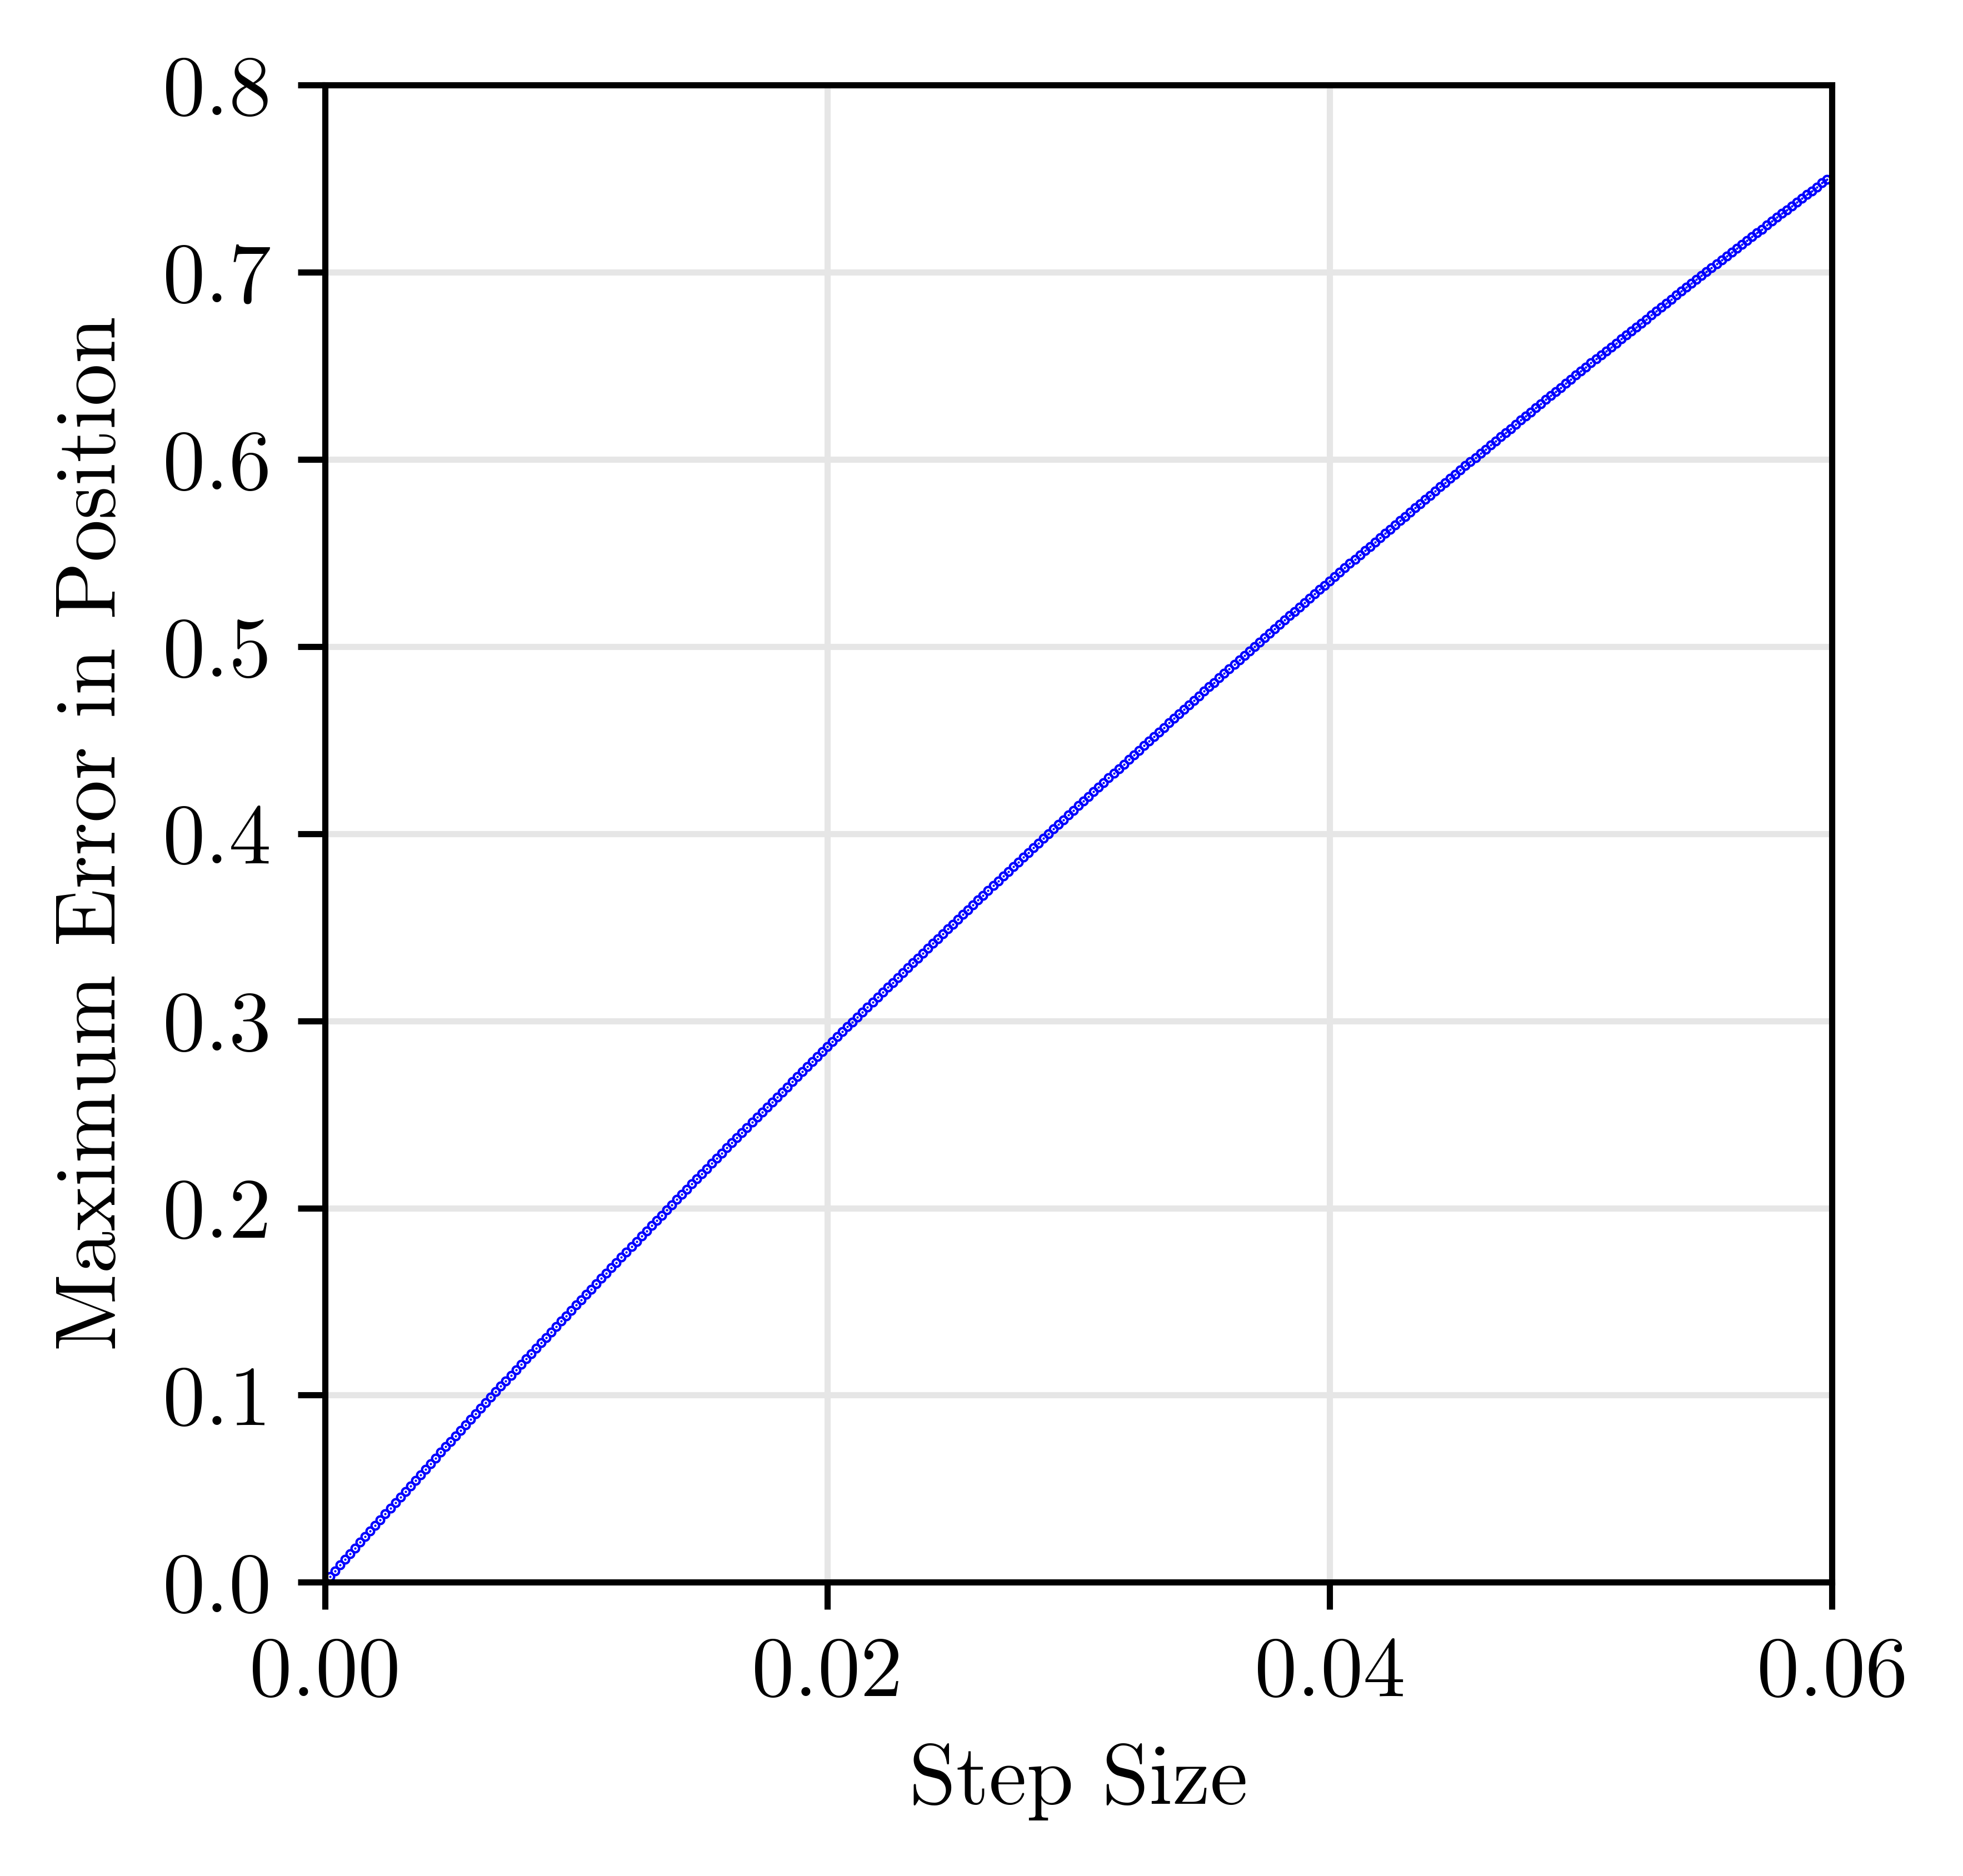
\includegraphics{implicit_euler_max_errors}\\
    \caption{(Left) The maximum error in positions obtained with the explicit Euler method for times in the interval $[0, 15)$, using step sizes in the range $[0.0002, 0.0058]$. (Right) The maximum error in positions obtained with the implicit Euler method, using step sizes in the range $[0.0002, 0.0058]$.}
    \label{fig:maxErrors}
\end{figure}

The error in position depends on the chosen step size. By plotting the maximum errors with varying step sizes, I found that the error for the explicit Euler method increases superlinearly as the step size increases, and that the error for the implicit Euler method increases sublinearly as the step size increases (see Figure \ref{fig:maxErrors}).

\section*{Part 2}

After adding the symplectic method to my program, I plotted a phase space diagram for the positions and velocities obtained with all three Euler methods, as well as those obtained analytically (see Figure \ref{fig:phaseSpace}). The trajectory for the explicit Euler method spirals outward, while the trajectory for the implicit Euler method spirals inward. The trajectory for the symplectic Euler method is an ellipse, and the trajectory for the analytic solution is a perfect circle.

I then plotted the energy obtained using the symplectic Euler method, which oscillates sinusoidally as $t$ increases (see Figure \ref{fig:energy2}). This corresponds to the motion toward and away from the origin that one undergoes while traversing the trajectory for the symplectic Euler method.

Finally, I plotted the positions obtained using the symplectic Euler method, as well as those obtained analytically, for times very far into the future (see Figure \ref{fig:positionsAndVelocities2}). This revealed that the oscillations predicted by the symplectic Euler method were slightly ahead of those predicted analytically.

\begin{figure}[H]
    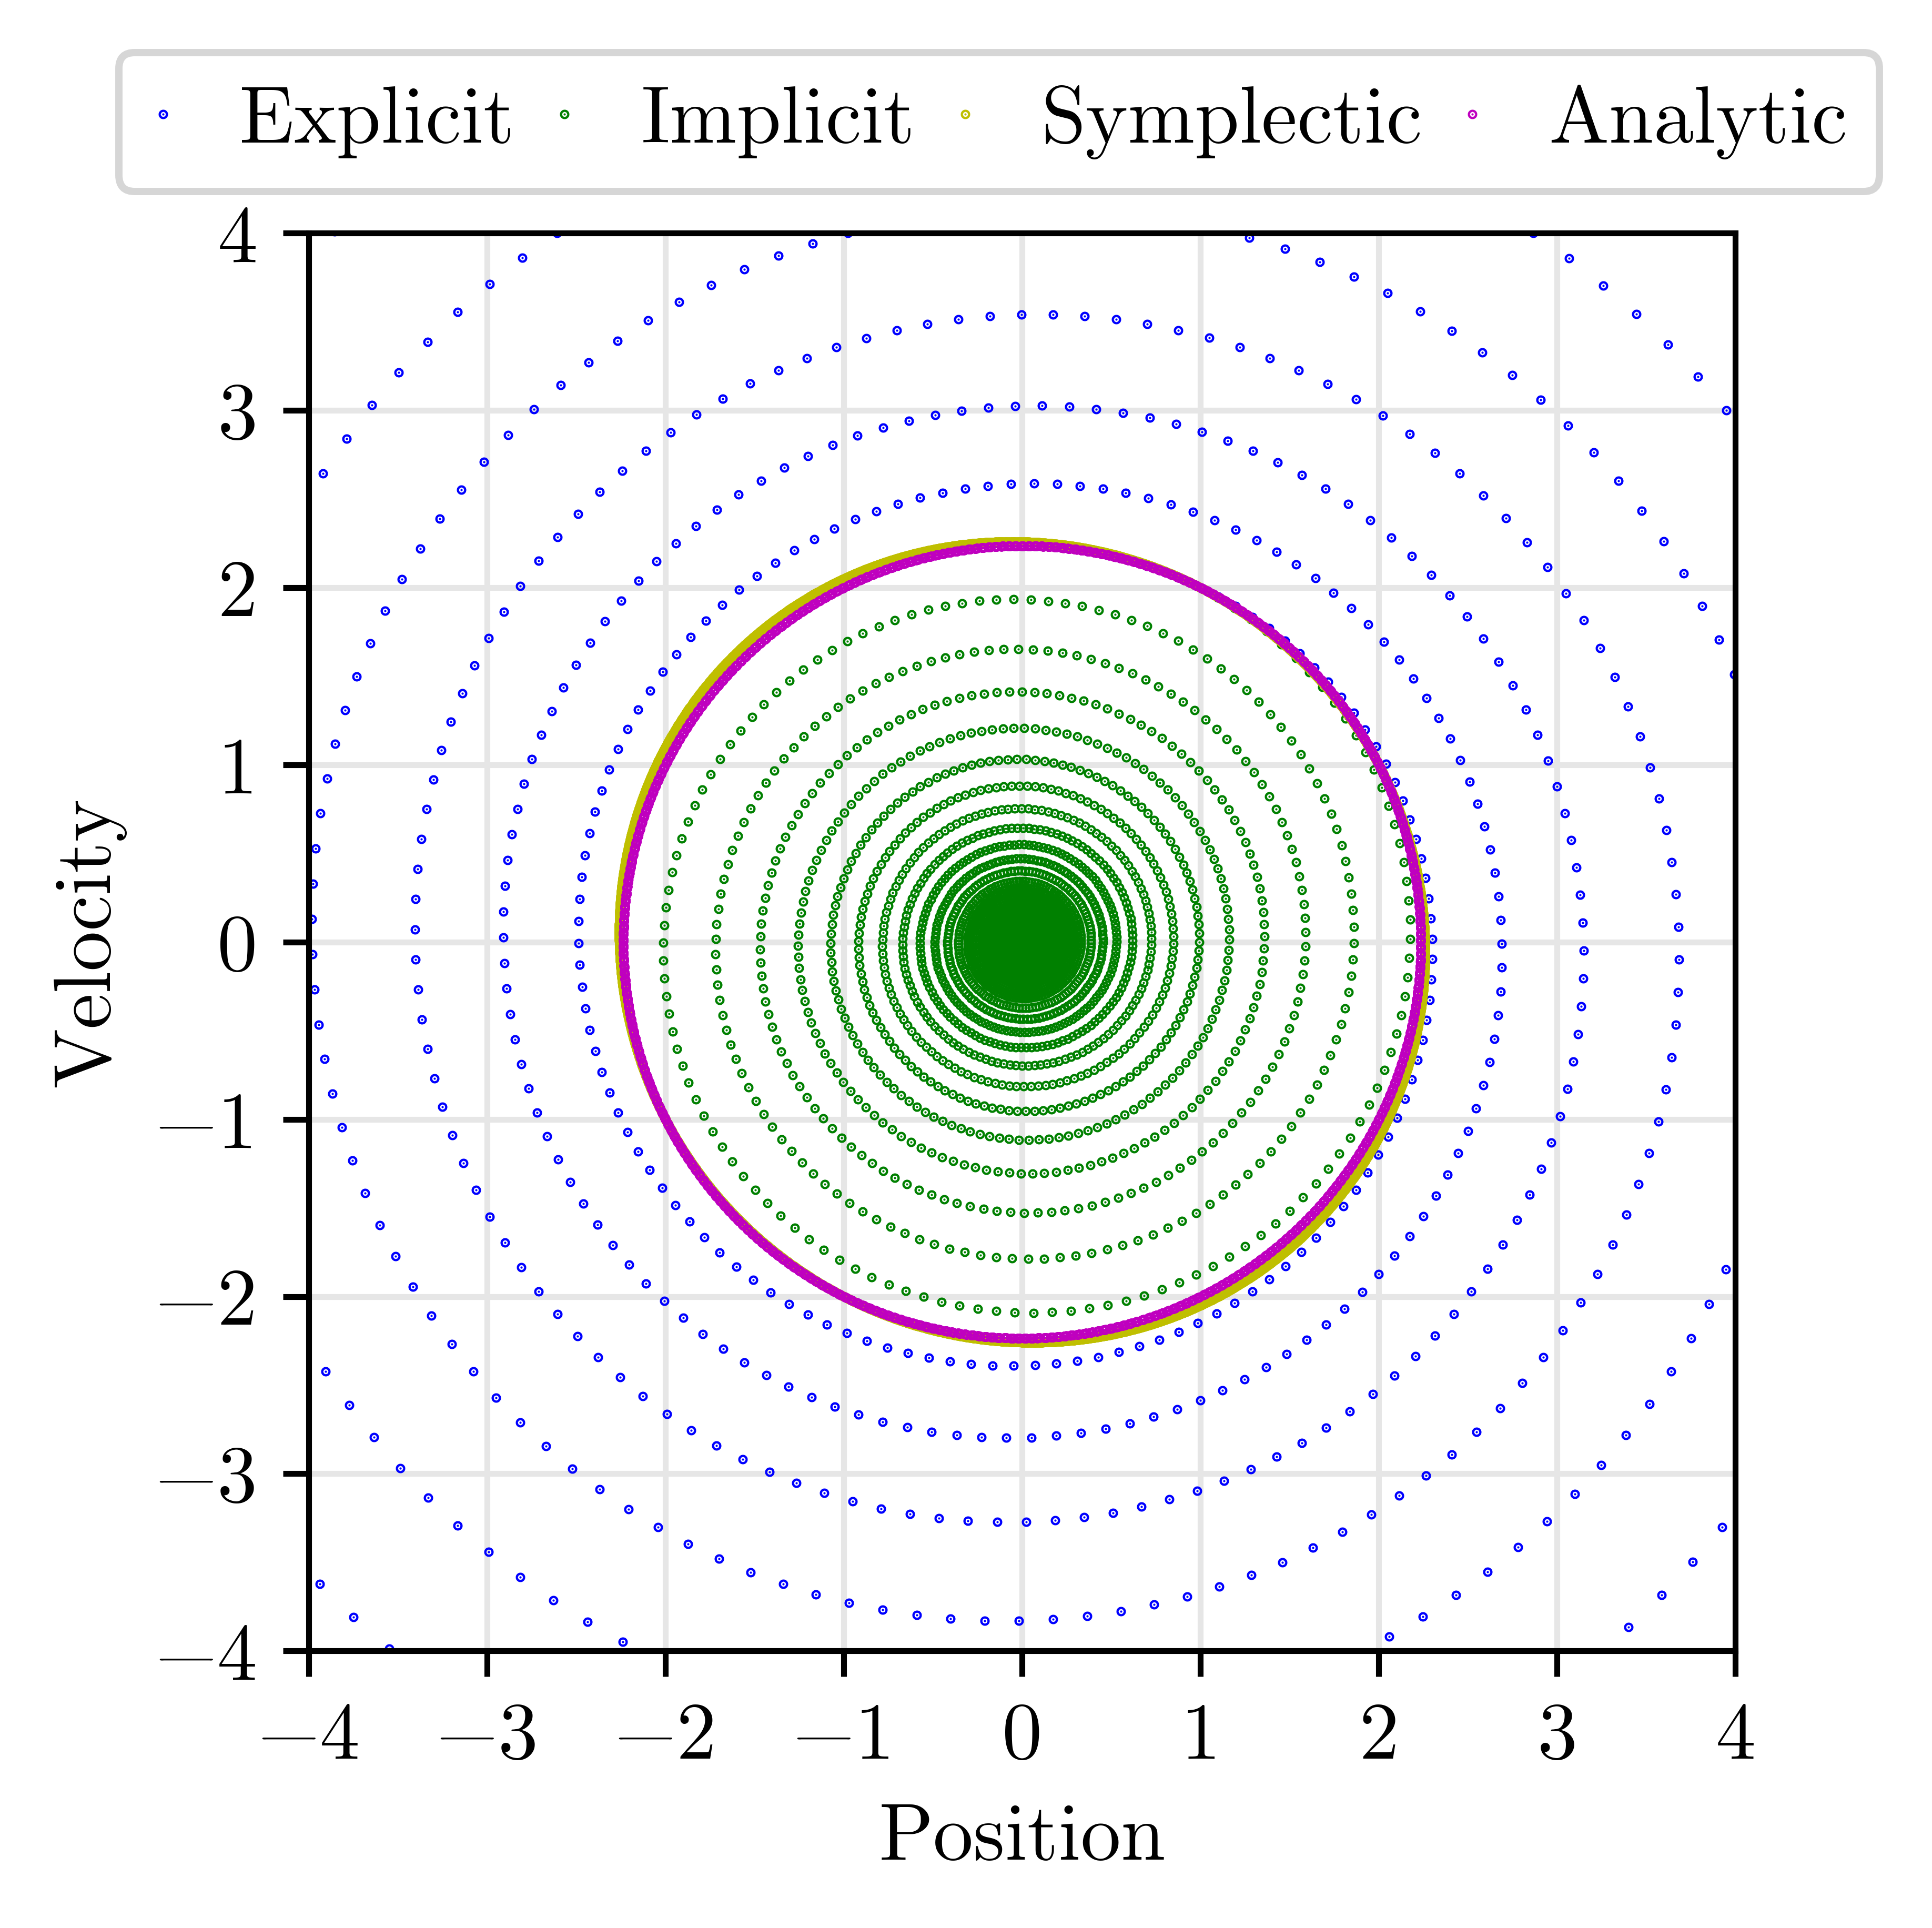
\includegraphics{phase_space}\\
    \caption{The phase space diagram for the positions and velocities obtained with all three Euler methods, using a step size of 0.05, as well as those obtained analytically.}
    \label{fig:phaseSpace}
\end{figure}

\vfill

\begin{figure}[H]
    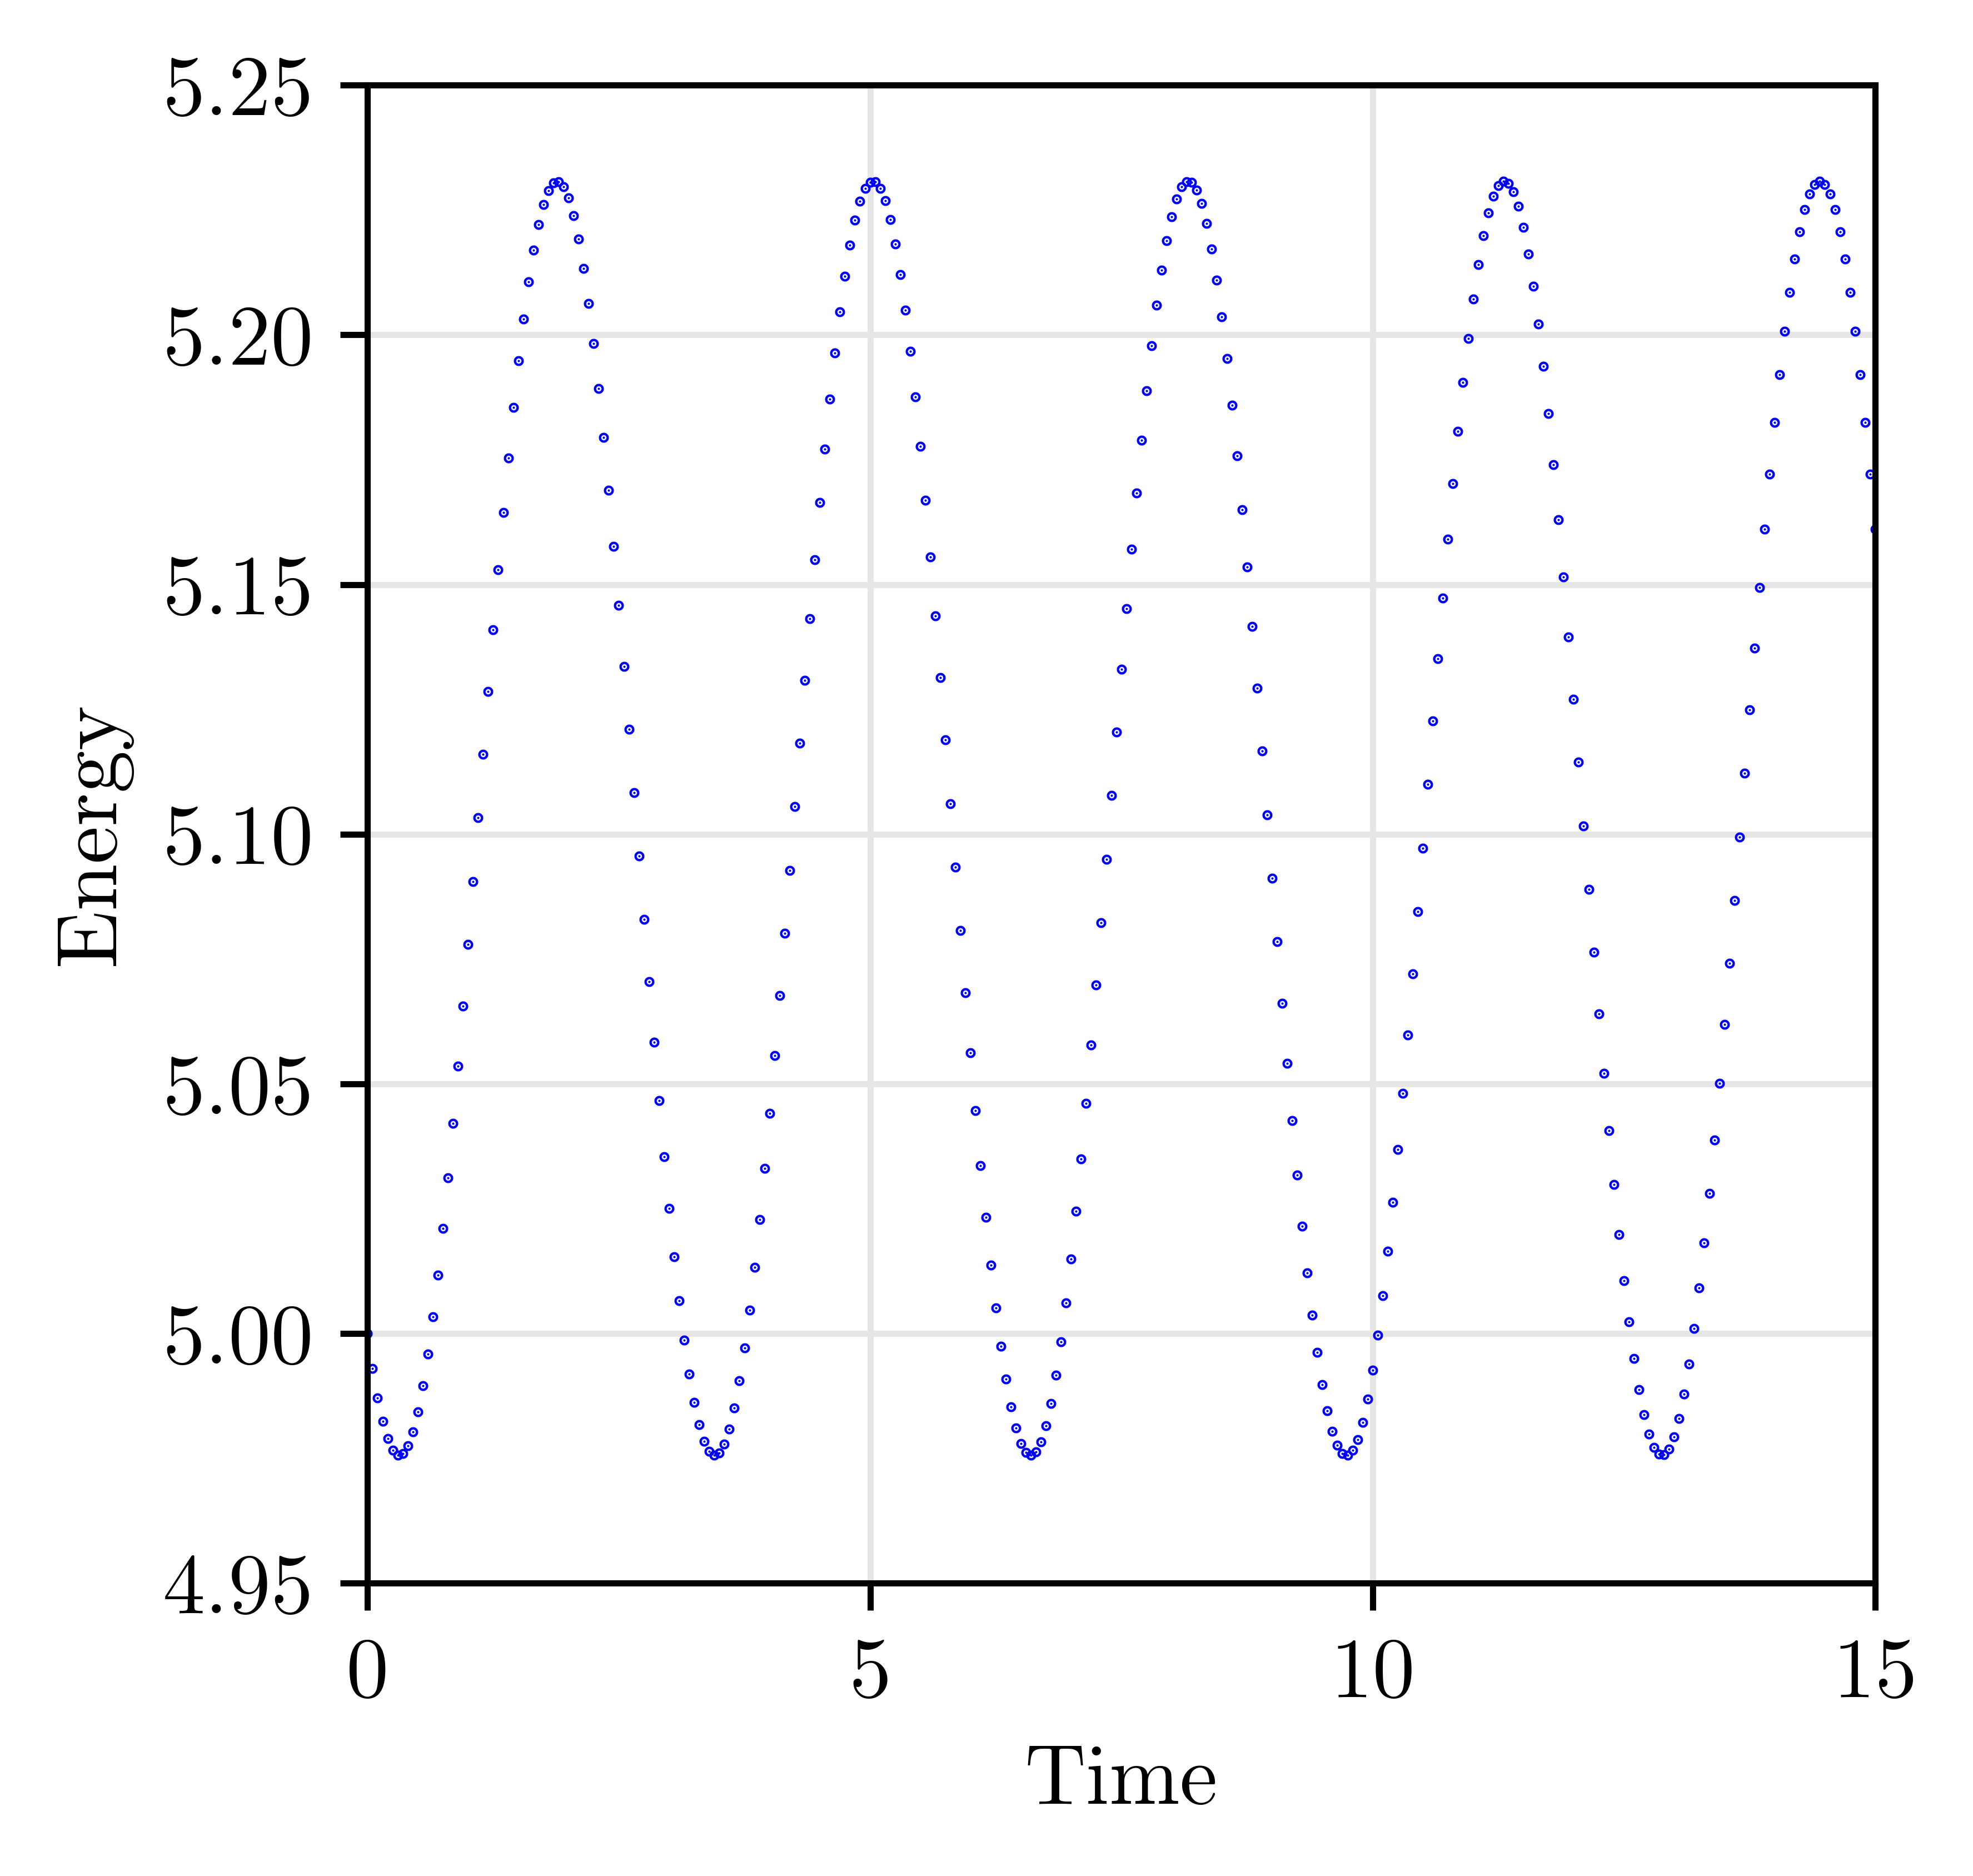
\includegraphics{symplectic_euler_energy}\\
    \caption{The energy obtained with the symplectic Euler method, using a step size of 0.05}
    \label{fig:energy2}
\end{figure}

\begin{figure}[H]
    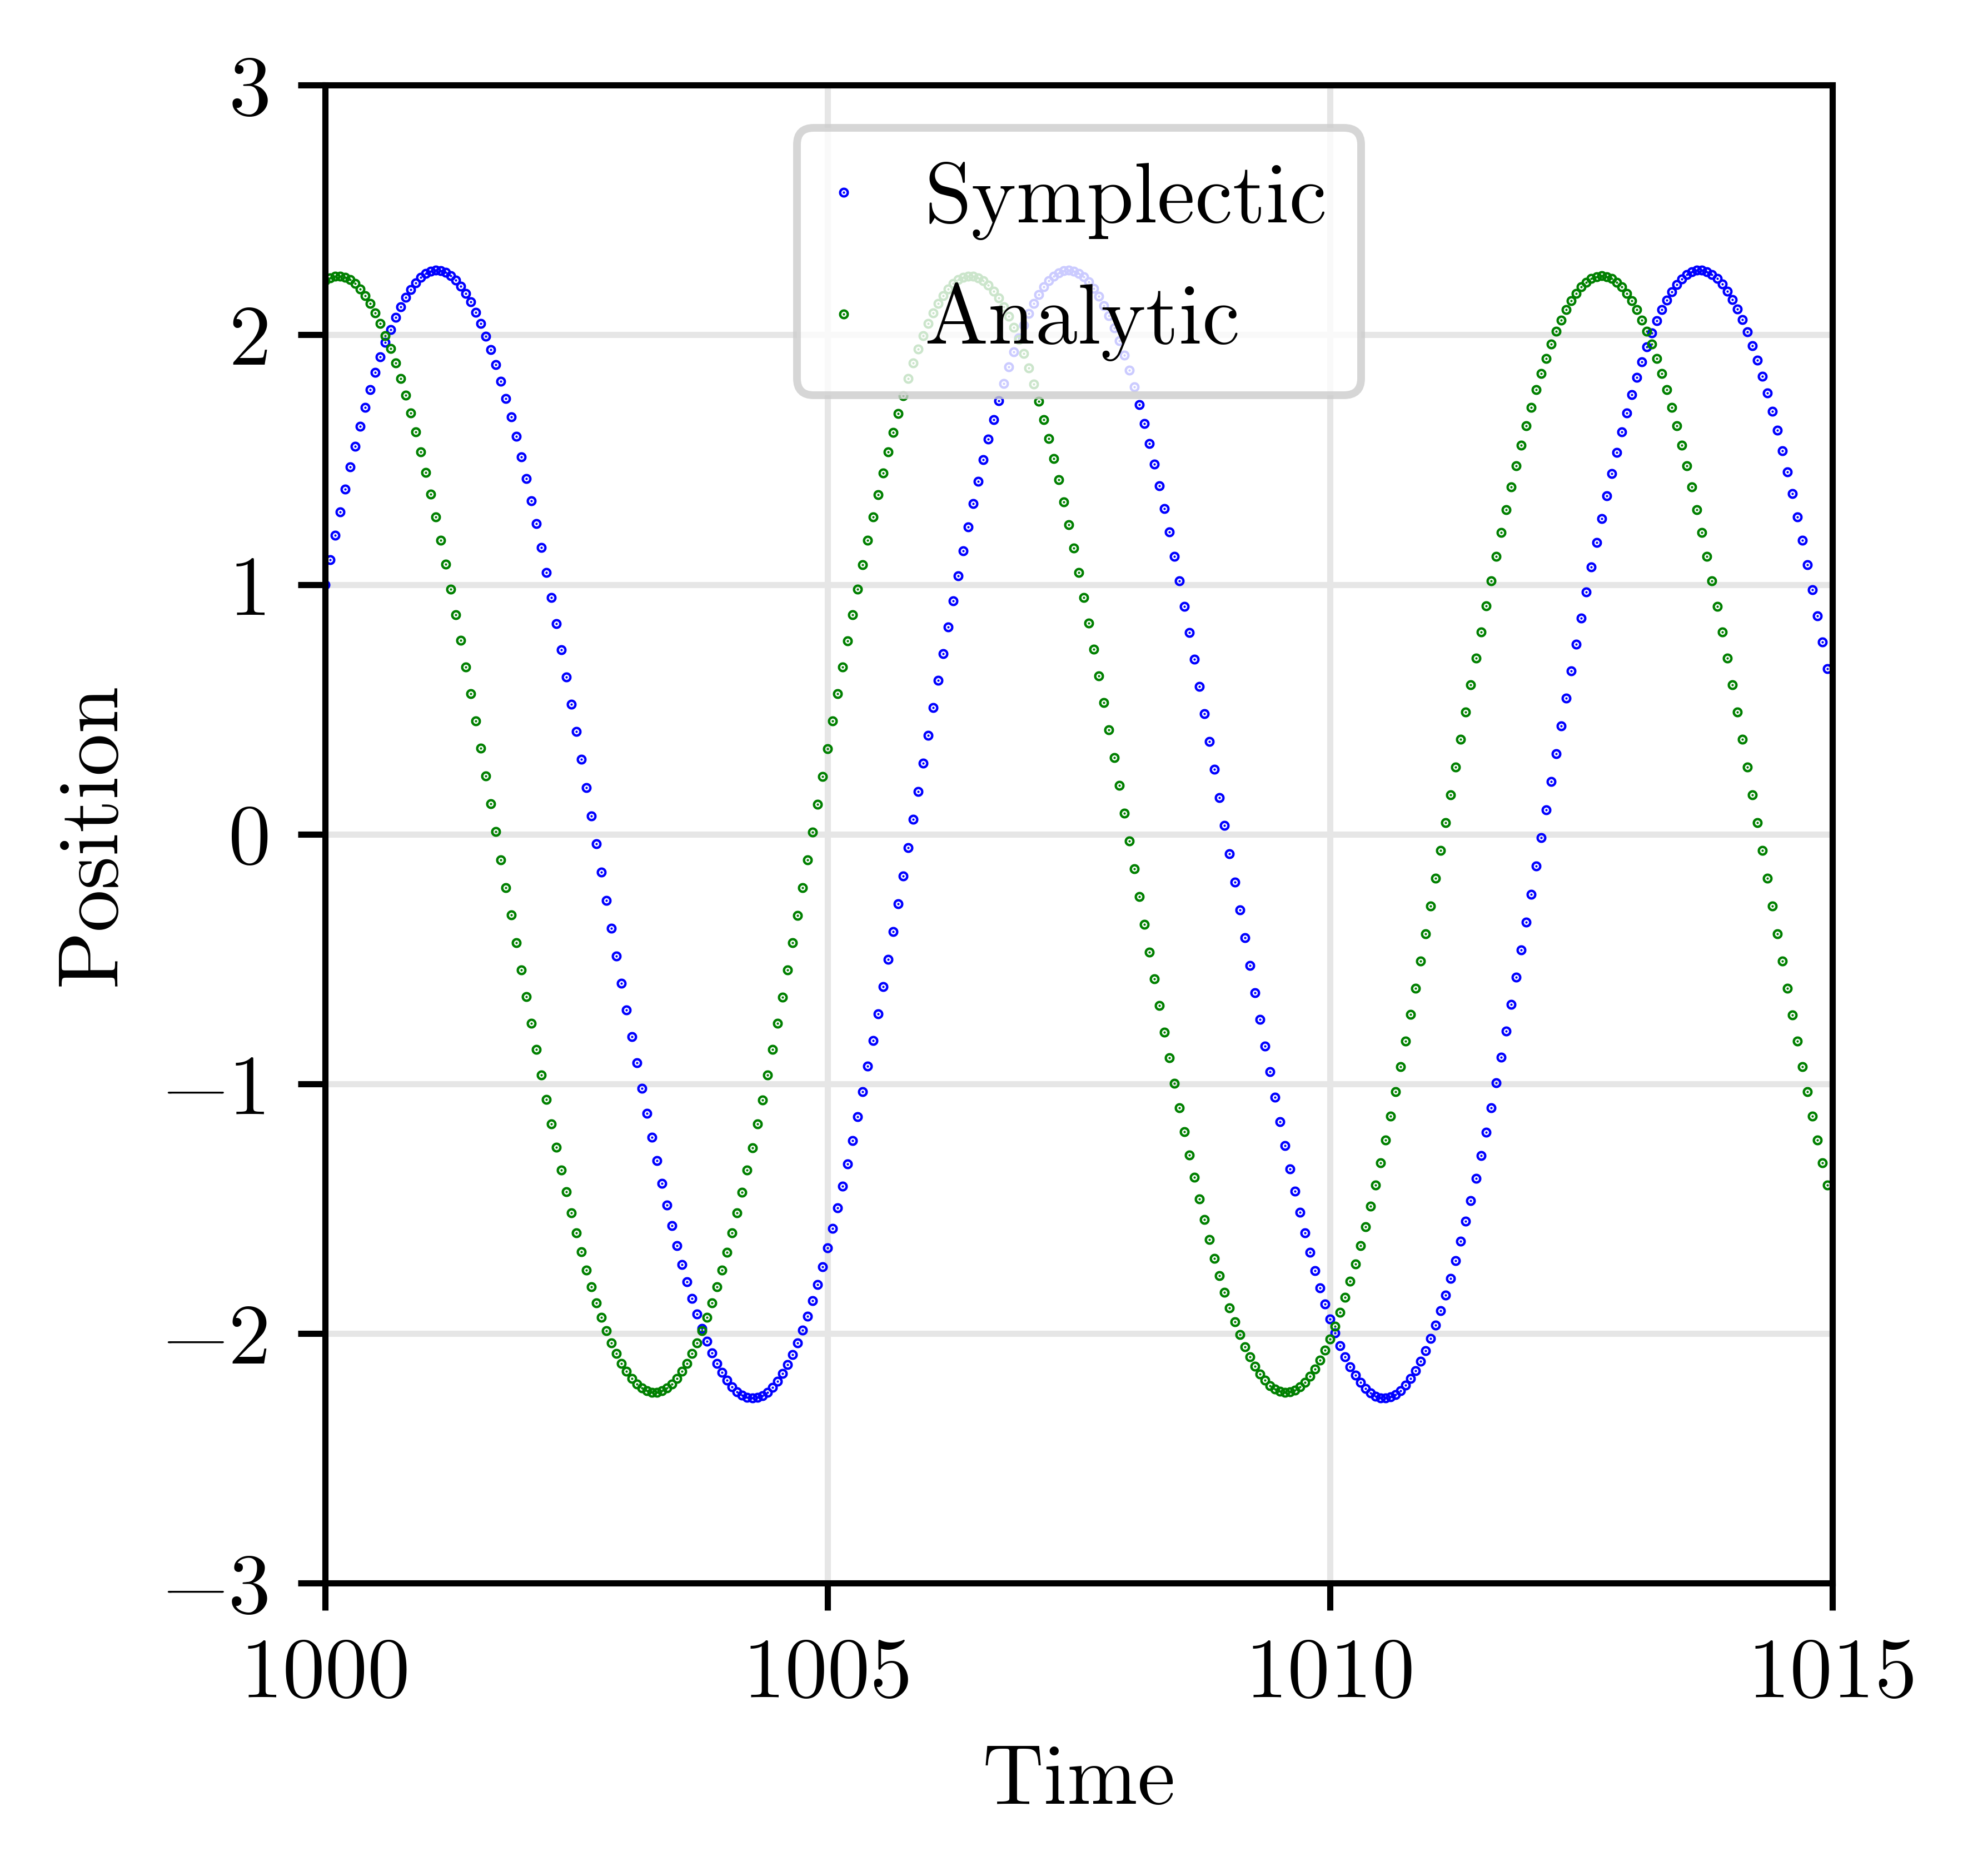
\includegraphics{symplectic_euler}\\
    \caption{The positions obtained with the symplectic Euler method, using a step size of 0.05, as well as the positions obtained analytically.}
    \label{fig:positionsAndVelocities2}
\end{figure}

\end{document}
